\documentclass[10pt,conference]{IEEEtran}

%%%%%%%%%%%%%%%%%%%%%%%%%%%%%%%%%%%%%%%%%%%%%%%%%%%%%%%%%%%%
%%%%%%%%%%%%%%%%%%%%%%%% PACKAGES %%%%%%%%%%%%%%%%%%%%%%%%%%
%%%%%%%%%%%%%%%%%%%%%%%%%%%%%%%%%%%%%%%%%%%%%%%%%%%%%%%%%%%%

\usepackage{amsmath}
\usepackage{amssymb}
\usepackage{graphicx}
\usepackage{booktabs}
\usepackage{multirow}
\usepackage{algorithm}
\usepackage{algpseudocode}
\usepackage{url}
\usepackage{cite}
\usepackage{array}
\usepackage{float}
\usepackage{subcaption}
\usepackage{xcolor}
\usepackage{enumitem}
\usepackage{bm}
\usepackage{tabularx}
\usepackage{tikz}
\usetikzlibrary{arrows.meta,shapes,fit,backgrounds,positioning,calc}
\graphicspath{{paper/figures/}}

%%%%%%%%%%%%%%%%%%%%%%%%%%%%%%%%%%%%%%%%%%%%%%%%%%%%%%%%%%%%
%%%%%%%%%%%%%%%%%%%%%%%% DOCUMENT %%%%%%%%%%%%%%%%%%%%%%%%%%
%%%%%%%%%%%%%%%%%%%%%%%%%%%%%%%%%%%%%%%%%%%%%%%%%%%%%%%%%%%%

\begin{document}

%%%%%%%%%%%%%%%%%%%%%%%%%%%%%%%%%%%%%%%%%%%%%%%%%%%%%%%%%%%%
%%%%%%%%%%%%%%%%%%%%%%%% TITLE %%%%%%%%%%%%%%%%%%%%%%%%%%%%%
%%%%%%%%%%%%%%%%%%%%%%%%%%%%%%%%%%%%%%%%%%%%%%%%%%%%%%%%%%%%

\title{Knowledge Graph Question Answering Using Reinforcement Learning}

\author{\IEEEauthorblockN{Ankit Rana}
\IEEEauthorblockA{Department of Computer Science and Engineering\\
NIT Calicut}
\and
\IEEEauthorblockN{Dr. Chandramani Chaudhary}
\IEEEauthorblockA{Department of Computer Science and Engineering\\
NIT Calicut}}

\maketitle

%%%%%%%%%%%%%%%%%%%%%%%%%%%%%%%%%%%%%%%%%%%%%%%%%%%%%%%%%%%%
%%%%%%%%%%%%%%%%%%%%%%%% ABSTRACT %%%%%%%%%%%%%%%%%%%%%%%%%%
%%%%%%%%%%%%%%%%%%%%%%%%%%%%%%%%%%%%%%%%%%%%%%%%%%%%%%%%%%%%

\begin{abstract}

% Abstract:
% - Problem
% - Existing limitations
% - Proposed framework
% - Key idea
% - Main results

Multi-hop Knowledge Graph Question Answering (KGQA) requires reasoning across complex relational paths in large-scale knowledge graphs. Existing systems commonly rely on static traversal strategies (e.g., fixed beam widths) that cause excessive graph exploration and severe error propagation, or reinforcement learning (RL) methods that optimize low-level relations, leading to massive action spaces and unstable training. To address these limitations, we propose an adaptive neuro-symbolic KGQA framework that dynamically regulates traversal-space expansion. The key idea is to decouple semantic reasoning planning from traversal optimization: we train a lightweight, high-level traversal controller that learns to adaptively regulate graph expansion widths—ranging from highly constrained to broad domain-guided exploration—conditioned on latent semantic confidence. Experimental evaluation on ComplexWebQuestions demonstrates that our adaptive traversal-control framework reduces average expanded edges from over 1,900 to just 14 per question, representing an order-of-magnitude efficiency gain while maintaining competitive multi-hop reasoning performance. Rather than relying on computationally heavy, frontier-scale language models, our approach targets a different point in the accuracy-efficiency-interpretability design space, offering highly transparent and lightweight neuro-symbolic reasoning.

\end{abstract}

%%%%%%%%%%%%%%%%%%%%%%%%%%%%%%%%%%%%%%%%%%%%%%%%%%%%%%%%%%%%
%%%%%%%%%%%%%%%%%%%%%%%% KEYWORDS %%%%%%%%%%%%%%%%%%%%%%%%%%
%%%%%%%%%%%%%%%%%%%%%%%%%%%%%%%%%%%%%%%%%%%%%%%%%%%%%%%%%%%%

\begin{IEEEkeywords}
Knowledge Graph Question Answering,
Multi-Hop Reasoning,
Reinforcement Learning,
Neuro-Symbolic Reasoning,
Graph Traversal,
Contrastive Learning
\end{IEEEkeywords}

%%%%%%%%%%%%%%%%%%%%%%%%%%%%%%%%%%%%%%%%%%%%%%%%%%%%%%%%%%%%
%%%%%%%%%%%%%%%%%%%%%%%% INTRODUCTION %%%%%%%%%%%%%%%%%%%%%%
%%%%%%%%%%%%%%%%%%%%%%%%%%%%%%%%%%%%%%%%%%%%%%%%%%%%%%%%%%%%

\section{Introduction}

\begin{figure*}[t]
\centering
% ============================================================
%  fig_kg.tex — Complex Multi-Hop Knowledge Graph (Spacious Spread)
%  Shows multiple entities, relation types, branching structure
%  Highlight path: Jerry Jones → Dallas Cowboys → Barry Switzer
% ============================================================

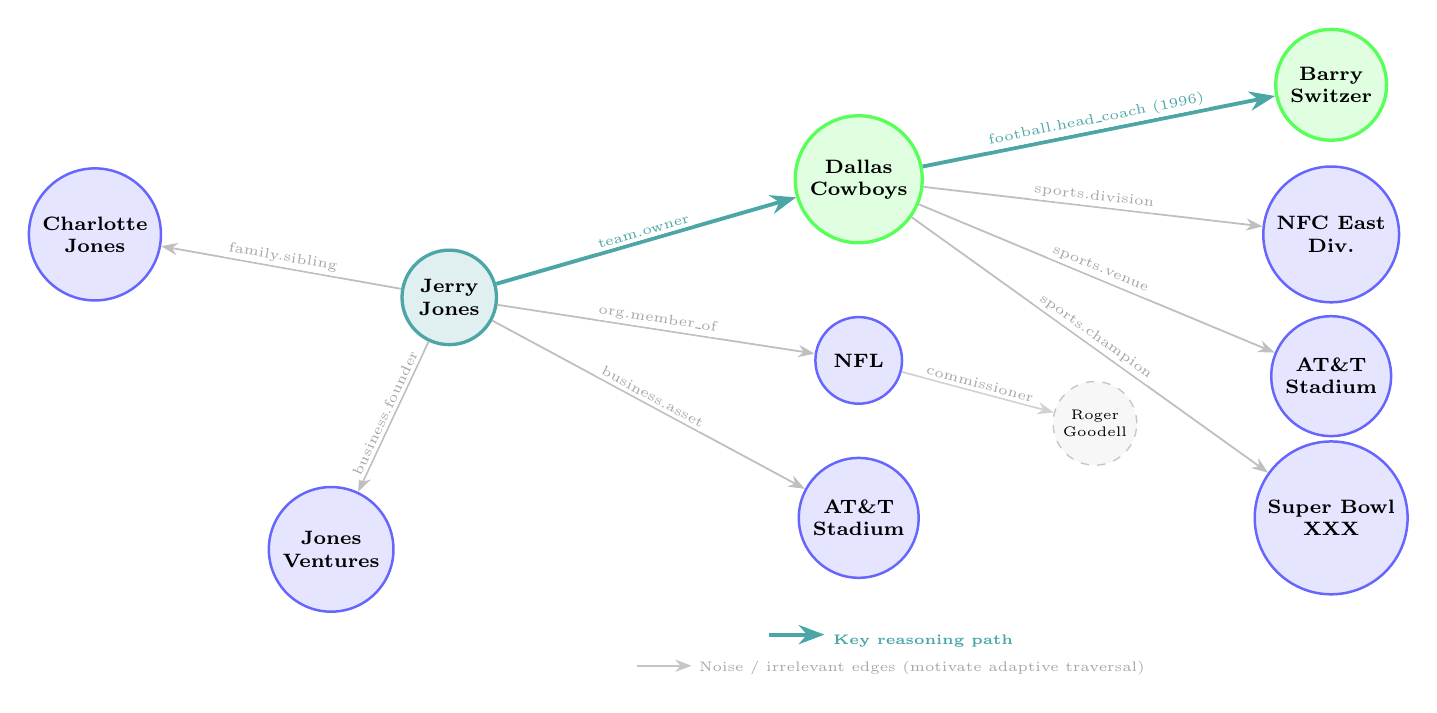
\begin{tikzpicture}[
  font=\small,
  >=Stealth,
  every node/.style={align=center},
  % Entity circles
  entity/.style={
    circle, draw=blue!60, fill=blue!10,
    inner sep=3pt, minimum size=1.1cm,
    font=\scriptsize\bfseries, line width=0.9pt
  },
  centity/.style={
    circle, draw=teal!70, fill=teal!12,
    inner sep=3pt, minimum size=1.2cm,
    font=\scriptsize\bfseries, line width=1.2pt
  },
  aentity/.style={
    circle, draw=green!65, fill=green!12,
    inner sep=3pt, minimum size=1.1cm,
    font=\scriptsize\bfseries, line width=1.2pt
  },
  noise/.style={
    circle, draw=gray!45, fill=gray!6,
    inner sep=2pt, minimum size=0.9cm,
    font=\tiny, line width=0.5pt, dashed
  },
  % Relation edge labels (Centered, sloped, small text)
  rel/.style={font=\tiny, fill=white, inner sep=1.2pt, text=gray!70},
  hrel/.style={font=\tiny, fill=white, inner sep=1.2pt, text=teal!70},
  % Arrows
  earr/.style={->, draw=gray!50, line width=0.65pt},
  harr/.style={->, draw=teal!70, line width=1.4pt},
]

% -------------------------------------------------------
% CENTER — Topic Entity
% -------------------------------------------------------
\node[centity]  (jj)   at (0,0)        {Jerry\\Jones};

% -------------------------------------------------------
% HOP 1 — Direct relations from Jerry Jones (Widely spaced)
% -------------------------------------------------------
\node[aentity]  (dc)   at (5.2, 1.5)   {Dallas\\Cowboys};   % CORRECT PATH
\node[entity]   (nfl)  at (5.2,-0.8)   {NFL};
\node[entity]   (atnt) at (5.2,-2.8)   {AT\&T\\Stadium};
\node[entity]   (biz)  at (-1.5,-3.2)  {Jones\\Ventures};
\node[entity]   (fam)  at (-4.5, 0.8)  {Charlotte\\Jones};

% Hop 1 edges (Sloped, perfectly centered, zero node overlap)
\draw[earr] (jj) -- node[rel,above,sloped,pos=0.5]{org.member\_of} (nfl);
\draw[earr] (jj) -- node[rel,above,sloped,pos=0.5]{business.asset} (atnt);
\draw[earr] (jj) -- node[rel,above,sloped,pos=0.5]{business.founder} (biz);
\draw[earr] (jj) -- node[rel,above,sloped,pos=0.5]{family.sibling} (fam);

% Hop 1 CORRECT edge
\draw[harr] (jj) -- node[hrel,above,sloped,pos=0.5]{team.owner} (dc);

% -------------------------------------------------------
% HOP 2 — Relations from Dallas Cowboys (Widely spaced at x=11.2)
% -------------------------------------------------------
\node[aentity]  (bs)   at (11.2, 2.7)   {Barry\\Switzer};    % ANSWER
\node[entity]   (eag)  at (11.2, 0.8)   {NFC East\\Div.};
\node[entity]   (att2) at (11.2,-1.0)   {AT\&T\\Stadium};
\node[entity]   (sb)   at (11.2,-2.8)   {Super Bowl\\XXX};

\draw[earr] (dc) -- node[rel,above,sloped,pos=0.5]{sports.division} (eag);
\draw[earr] (dc) -- node[rel,above,sloped,pos=0.5]{sports.venue} (att2);
\draw[earr] (dc) -- node[rel,above,sloped,pos=0.5]{sports.champion} (sb);

% Hop 2 CORRECT edge
\draw[harr] (dc) -- node[hrel,above,sloped,pos=0.5]{football.head\_coach (1996)} (bs);

% -------------------------------------------------------
% HOP 2 — Relations from NFL (noise branch)
% Roger Goodell is placed to the right of NFL to avoid AT&T Stadium (at x=5.2)
% -------------------------------------------------------
\node[noise]  (n2)  at (8.2,-1.6)  {Roger\\Goodell};
\draw[earr, draw=gray!35] (nfl) -- node[rel,above,sloped,pos=0.5]{commissioner} (n2);

% -------------------------------------------------------
% LEGEND (Centered at x=5.6)
% -------------------------------------------------------
\node[font=\tiny\bfseries, text=teal!70] at (5.6,-4.3) {%
  \tikz\draw[harr](-0.2,0)--(0.5,0); Key reasoning path};
\node[font=\tiny, text=gray!70] at (5.6,-4.7) {%
  \tikz\draw[earr, gray!45](-0.2,0)--(0.5,0); Noise / irrelevant edges (motivate adaptive traversal)};

\end{tikzpicture}

\caption{Multi-hop KG reasoning trace from CWQ. Question: \textit{``Who was the 1996 coach of the team owned by Jerry Jones?''} Teal arrows show the correct 2-hop path: \textit{team.owner} $\to$ Dallas Cowboys $\to$ \textit{football.hist\_coach} $\to$ Barry Switzer. Grey dashed nodes/edges are noise neighbours (org membership, business assets, family relations, stadium links) that static traversal must explore, motivating adaptive traversal-control.}
\label{fig:kg}
\end{figure*}

Knowledge Graph Question Answering (KGQA) enables interpretable reasoning over structured relational data. However, answering compositional questions remains highly challenging; as reasoning depth increases, traversal complexity grows exponentially due to the massive branching factor of KGs like Freebase, resulting in intractable exploration spaces. As illustrated in Figure~\ref{fig:kg}, static traversal methods must explore numerous irrelevant neighboring nodes (e.g., stadium links, business assets, family relations), leading to an exponential traversal-space explosion.

Recent KGQA research increasingly relies on frontier-scale large language models (LLMs) to navigate complex symbolic structures. While these systems achieve remarkable accuracy, they incur high computational overhead, substantial memory footprints, and rely on opaque, implicit reasoning pathways. In contrast, we investigate an alternative design trade-off, asking whether adaptive symbolic traversal and reinforcement learning can achieve competitive reasoning behavior using lightweight, transformer-based components. Rather than competing directly on raw parametric scale, we prioritize resource efficiency, low-latency execution, and fully explicit, transparent graph traversal.

While recent reinforcement learning (RL) methods formulate multi-hop reasoning as a sequential decision-making problem, they commonly direct the policy to optimize low-level graph traversal actions (i.e., directly selecting specific relation IDs or neighboring nodes at each step). In large-scale KGs with thousands of unique relations, this formulation leads to massive action spaces, severe reward sparsity, and highly unstable policy optimization. Effective multi-hop reasoning instead requires adaptive traversal behavior conditioned on semantic confidence and question complexity.

To address these limitations, we propose the key idea of \emph{decoupling semantic reasoning planning from graph traversal optimization}. In our framework, a semantic planner predicts relation paths, while the RL traversal controller focuses solely on selecting search expansion widths rather than individual relations. By restricting the RL action space to a few high-level exploration controls, we aim to simplify policy learning and promote stable training. Specifically, the RL policy selects among four high-level actions—\textsc{Constrained}, \textsc{Moderate}, \textsc{Exploratory}, and \textsc{Terminate}—to regulate graph exploration on-the-fly. Finally, a Candidate Disambiguation \& Selection (CDS) ranker refines the final answer.

The main contributions of this work are summarized as follows:

\begin{itemize}

\item \textbf{Semantic Planner:} A multi-task reasoning module that predicts cross-hop relation trajectories and dynamic stop signals, while outputting a scalar confidence score to capture question complexity.

\item \textbf{RL Traversal Controller:} A reinforcement learning policy that operates over a compact, high-level action space to adaptively regulate graph exploration width (ranging from highly constrained to broad search) based on the planner's confidence.

\item \textbf{STRL (Semantic-Teacher RL):} A curriculum-based training variant that aligns RL traversal states with target relation embeddings via contrastive InfoNCE supervision, aiming to mitigate the risk of policy collapse and semantic drift.

\item \textbf{CDS Reranker:} A multi-stage cascading reranking framework (Cascading Dust Separator) that progressively filters candidate search noise using a hierarchy of bi-encoders, path-aware classifiers, and DPO-aligned generative judges to promote high precision.

\item Experimental evaluation on ComplexWebQuestions demonstrates that our adaptive traversal-control framework reduces average expanded edges from over 1,900 to just 14 per question, representing an order-of-magnitude efficiency gain and competitive reasoning accuracy while maintaining full symbolic transparency and interpretability.

\end{itemize}

%%%%%%%%%%%%%%%%%%%%%%%%%%%%%%%%%%%%%%%%%%%%%%%%%%%%%%%%%%%%
%%%%%%%%%%%%%%%%%%%%%%%% RELATED WORK %%%%%%%%%%%%%%%%%%%%%%
%%%%%%%%%%%%%%%%%%%%%%%%%%%%%%%%%%%%%%%%%%%%%%%%%%%%%%%%%%%%

\section{Related Work}

Knowledge Graph Question Answering (KGQA) has been extensively studied using multiple reasoning paradigms. In this section, we discuss the major categories of existing approaches and position our adaptive traversal framework within the literature.

\subsection{Reinforcement Learning Based KGQA}
Iterative reasoning systems model KGQA as a sequential traversal process over graph structures \cite{xiong2017deeppath, das2017go, lin2018multi, sun2018open, xian2019reinforcement, sun2019pullnet, wang2020reasoning}. Reinforcement learning (RL) methods further optimize these trajectories by framing reasoning as a Markov Decision Process (MDP). However, traditional RL-based KGQA systems directly optimize low-level graph actions (e.g., specific relation IDs or neighboring entities). Consequently, these methods frequently suffer from extremely large action spaces, sparse rewards, and unstable policy optimization, limiting their utility to smaller graph sub-structures.

\paragraph*{Contrast with Relation-Level RL (DeepPath \& MINERVA)}
Conventional RL-based KGQA approaches, pioneered by DeepPath \cite{xiong2017deeppath} and MINERVA \cite{das2017go}, formulate graph traversal by training an agent whose action space consists of all possible outgoing relations (or neighbor entities) at each hop. In massive KGs like Freebase, this action vocabulary exceeds tens of thousands of items, resulting in severe optimization challenges, sparse rewards, and policy instability. Our method fundamentally differs by moving relation selection to a supervised semantic planner. The RL agent's action space is reduced to just four abstract traversal-width controls, transforming a high-dimensional path-finding problem into a low-dimensional exploration-control task. This structural decoupling is designed to serve as the key driver of our framework's training stability and traversal efficiency.

\subsection{Neuro-Symbolic KGQA}
Early KGQA systems primarily relied on semantic parsing techniques \cite{yih2015semantic, bao2016constraint} that transformed natural language questions into executable logical forms, which provide strong interpretability but require expensive annotation and struggle to scale. Embedding-based methods introduce continuous vector-space representations for entities and relations \cite{bordes2013translating, yang2014embedding, trouillon2016complex, sun2019rotate, saxena2020improving, sun2020faithful}, but lack explicit reasoning transparency. More recently, hybrid neuro-symbolic systems, including Graph Neural Networks (GNNs) \cite{kipf2016semi, velickovic2017graph, schlichtkrull2018modeling, yasunaga2021qa, zhang2022subgraph} and transformer-based structural reasoning frameworks \cite{liu2019roberta, jiang2023structgpt, wang2023knowledgpt, luo2024reasoning}, model graph neighborhoods to improve semantic generalization. Despite these improvements, most neuro-symbolic frameworks still rely on static, predefined traversal heuristics (e.g., fixed beam widths) during graph exploration, leading to excessive search cost or error propagation on highly complex or ambiguous questions.

\subsection{Large Language Model Guided KGQA}
Recent literature increasingly emphasizes the use of frontier-scale large language models (LLMs) such as GPT-4 \cite{achiam2023gpt} and Llama \cite{touvron2023llama}, alongside robust conversational and agentic graph reasoning frameworks \cite{christmann2024reign, chen2024search, chen2025drkg, zhao2025enrich}. These systems often employ retrieval-augmented reasoning and multi-agent prompting to navigate symbolic structures. While LLM-based systems achieve strong raw accuracy, they operate on the computationally expensive end of the efficiency spectrum and rely on implicit reasoning steps. In this work, rather than competing directly on raw parametric capacity, we investigate a different design trade-off. Our proposed framework prioritizes explicit symbolic traversal and interpretable traversal-width control using comparatively lightweight and highly reproducible transformer encoders, achieving high traversal transparency and order-of-magnitude efficiency gains.

\subsection{Summary of Differences}
Unlike existing RL-based methods that directly choose relation actions over huge spaces, or neuro-symbolic methods that employ static traversal widths, our framework decouples semantic path prediction from traversal-width control. This reduces RL complexity, mitigates optimization instability, and supports highly efficient and adaptive symbolic reasoning.

%%%%%%%%%%%%%%%%%%%%%%%%%%%%%%%%%%%%%%%%%%%%%%%%%%%%%%%%%%%%
%%%%%%%%%%%%%%%%%%%%%%%% PRELIMINARIES %%%%%%%%%%%%%%%%%%%%%
%%%%%%%%%%%%%%%%%%%%%%%%%%%%%%%%%%%%%%%%%%%%%%%%%%%%%%%%%%%%

\section{Preliminaries}

We define the core formalisms used throughout the paper.

\subsection{Knowledge Graph}

A knowledge graph $\mathcal{G}=(\mathcal{E},\mathcal{R},\mathcal{T})$ consists of entity set $\mathcal{E}$, relation set $\mathcal{R}$, and relational triples $\mathcal{T}$. Each triple $(e_s,r,e_o)$ encodes that subject $e_s$ connects to object $e_o$ via relation $r$. The neighborhood of an entity is $\mathcal{N}(e) = \{ e' \mid (e,r,e') \in \mathcal{T} \}$. Real-world KGs such as Freebase contain millions of entities with dense relational structure, yielding large branching factors during traversal.

\subsection{Multi-Hop KGQA}

Given question $q$ and topic entity $e_0$, the task is to retrieve answer set $\mathcal{A}=\{a_1,\dots,a_n\}$ via sequential traversal $e_0 \xrightarrow{r_1} e_1 \xrightarrow{r_2} \cdots \xrightarrow{r_h} e_h$. At each hop, the candidate set expands as $E_{h+1} = \{ e' \mid (e,r,e') \in \mathcal{T},\, e \in E_h \}$. For an average graph branching factor $b$ and reasoning depth $h$, the traversal-space complexity grows exponentially as $\mathcal{O}(b^h)$, making exhaustive expansion infeasible for deep reasoning chains. The multi-hop reasoning trace shown in Figure~\ref{fig:kg} highlights how this traversal-space expansion introduces substantial candidate noise (dashed nodes and edges) that a static traversal method must exhaustively explore.

Following standard KGQA evaluation practice on CWQ, we assume topic entities are provided by dataset annotations. Entity linking is therefore out of scope for this work.


%%%%%%%%%%%%%%%%%%%%%%%%%%%%%%%%%%%%%%%%%%%%%%%%%%%%%%%%%%%%
%%%%%%%%%%%%%%%%%%%%%%%% PROBLEM FORMULATION %%%%%%%%%%%%%%%
%%%%%%%%%%%%%%%%%%%%%%%%%%%%%%%%%%%%%%%%%%%%%%%%%%%%%%%%%%%%

\section{Problem Formulation}
\label{sec:probform}

The core challenge in multi-hop KGQA is traversing complex relational paths without succumbing to traversal-space explosion. Static traversal strategies apply an identical, fixed expansion width to all questions regardless of semantic complexity, causing excessive over-exploration on simple queries and severe under-exploration on ambiguous ones. To address this, we formulate traversal-space control as a sequential decision-making problem under a Markov Decision Process (MDP), defined by the tuple $\mathcal{M}=(\mathcal{S},\mathcal{A},\mathcal{P},\mathcal{R})$, where:

\begin{itemize}
\item \textbf{State Space $\mathcal{S}$}: At each reasoning step $t$, the state $s_t \in \mathcal{S}$ represents the latent context of the question and the traversed path, encoding the reasoning state of the query and the current relational path history.
\item \textbf{Action Space $\mathcal{A}$}: Rather than selecting relation-level actions directly, the action space consists of abstract traversal-width controls that regulate neighborhood expansion:
\begin{equation}
\mathcal{A} = \{ a_{\text{constrained}},\; a_{\text{moderate}},\; a_{\text{exploratory}},\; a_{\text{terminate}} \}
\end{equation}
Specifically, $a_{\text{constrained}}$ restricts traversal to the single top relation (beam width $k=1$), $a_{\text{moderate}}$ expands traversal to a moderate relational width ($k=5$), $a_{\text{exploratory}}$ performs a broad search over semantically relevant neighborhoods ($k=50$), and $a_{\text{terminate}}$ terminates the traversal.
\item \textbf{Transition Probability $\mathcal{P}$}: The transition function $\mathcal{P}(s_{t+1} \mid s_t, a_t)$ defines the probability of moving to the next latent reasoning state $s_{t+1}$ given the current state $s_t$ and the selected width-expansion action $a_t$. Concretely, after action $a_t$ determines beam width $k$, the entity frontier $E_t$ is expanded to $E_{t+1}$ by following the top-$k$ predicted relations in $\mathcal{G}$; the next state $s_{t+1} = x_{t+1}$ uses the planner's pre-computed representation for hop $t{+}1$. CWQ questions may have multiple valid answer entities; $Acc_t$ is therefore set to 1 if \emph{any} gold answer entity is present in the current frontier $E_t$, and 0 otherwise. At evaluation, Hits@1 is reported against the first listed gold answer following standard CWQ protocol.
\item \textbf{Reward Function $\mathcal{R}$}: The step-level reward $R_t$ balances path accessibility with search space efficiency:
\begin{equation}
R_t = \alpha\, Acc_t - \beta\, Cost_t - \gamma\, Width_t
\end{equation}
where $Acc_t \in \{0, 1\}$ denotes answer accessibility (1 if the gold entity remains reachable, 0 otherwise), $Cost_t$ measures the volume of expanded graph edges, and $Width_t$ represents the action-determined beam width. The width penalty $\gamma\, Width_t$ explicitly penalizes broader search widths, helping to prevent the policy from consistently selecting broad exploratory actions when narrower, more confident paths are available.
\end{itemize}

The optimization objective is to learn a traversal-control policy $\pi(a_t \mid s_t)$ that maximizes the expected discounted cumulative return:
\begin{equation}
J(\pi) = \mathbb{E}_{\tau \sim \pi}\!\left[\sum_{t=0}^{T} \gamma_{\text{discount}}^{t}\, R_t\right]
\end{equation}
where $\gamma_{\text{discount}} \in [0, 1)$ is the discount factor. Operating over this compact action space of search widths rather than high-dimensional relation IDs keeps the policy space small, designed to support stable optimization behavior regardless of the knowledge graph's vocabulary size.

%%%%%%%%%%%%%%%%%%%%%%%%%%%%%%%%%%%%%%%%%%%%%%%%%%%%%%%%%%%%
%%%%%%%%%%%%%%%%%%%%%%%% METHODOLOGY %%%%%%%%%%%%%%%%%%%%%%%
%%%%%%%%%%%%%%%%%%%%%%%%%%%%%%%%%%%%%%%%%%%%%%%%%%%%%%%%%%%%

\section{Methodology}

The proposed framework operates through three sequential stages. \textbf{Stage~I} (Semantic Planner) is trained via supervised learning to predict relational paths and a semantic confidence score. \textbf{Stage~II} (RL Traversal Controller) learns a traversal-control policy over the frozen representations of Stage~I. \textbf{Stage~III} (Candidate Disambiguation \& Selection, CDS) ranks the traversal outputs to select the final answer. An overview of this architecture is illustrated in Figure~\ref{fig:arch}.

\begin{figure*}[t]
\centering
% =====================================================================
%  fig_detailed_dataflow.tex — End-to-End Hierarchical KGQA Dataflow
% =====================================================================

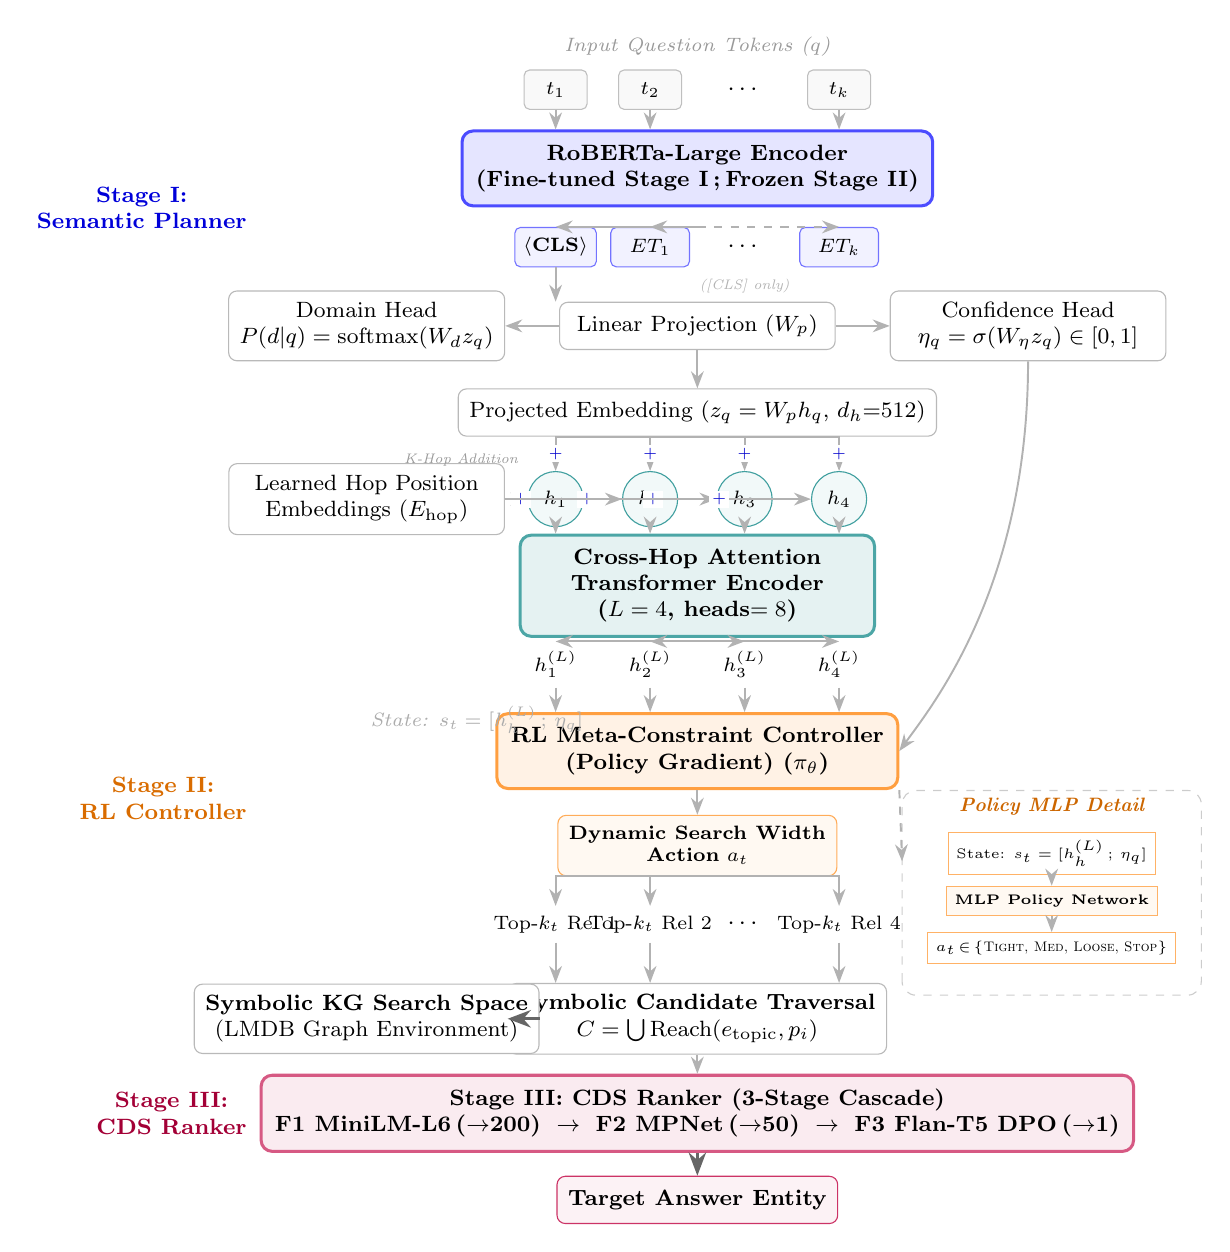
\begin{tikzpicture}[
  font=\small,
  >=Stealth,
  every node/.style={align=center},
  % ---- box styles ----
  tokenbox/.style={
    rectangle, rounded corners=2pt,
    draw=gray!50, fill=gray!5,
    inner sep=3pt, minimum width=0.8cm, minimum height=0.5cm,
    font=\scriptsize
  },
  embbox/.style={
    rectangle, rounded corners=2pt,
    draw=blue!55, fill=blue!5,
    inner sep=3pt, minimum width=1.0cm, minimum height=0.5cm,
    font=\scriptsize\bfseries
  },
  bluebox/.style={
    rectangle, rounded corners=4pt,
    draw=blue!70, fill=blue!10,
    inner sep=5pt, minimum width=4.5cm, minimum height=0.7cm,
    line width=1.1pt, font=\footnotesize\bfseries
  },
  qbox/.style={
    rectangle, rounded corners=3pt,
    draw=gray!55, fill=white,
    inner sep=4pt, minimum width=3.5cm, minimum height=0.6cm,
    font=\footnotesize
  },
  tealbox/.style={
    rectangle, rounded corners=4pt,
    draw=teal!70, fill=teal!10,
    inner sep=5pt, minimum width=4.5cm, minimum height=0.7cm,
    line width=1.1pt, font=\footnotesize\bfseries
  },
  ppobox/.style={
    rectangle, rounded corners=4pt,
    draw=orange!75, fill=orange!10,
    inner sep=5pt, minimum width=4.5cm, minimum height=0.7cm,
    line width=1.1pt, font=\footnotesize\bfseries
  },
  cdsbox/.style={
    rectangle, rounded corners=4pt,
    draw=purple!65, fill=purple!8,
    inner sep=5pt, minimum width=4.5cm, minimum height=0.7cm,
    line width=1.1pt, font=\footnotesize\bfseries
  },
  circlehop/.style={
    circle, draw=teal!75, fill=teal!5,
    inner sep=2pt, minimum size=0.7cm,
    font=\scriptsize\bfseries
  },
  actbox/.style={
    rectangle, rounded corners=3pt,
    draw=orange!65, fill=orange!5,
    inner sep=4pt, minimum width=3.5cm, minimum height=0.6cm,
    font=\scriptsize
  },
  arr/.style={->, draw=gray!60, line width=0.7pt},
  Arr/.style={->, draw=black!60, line width=1.2pt},
  dashedarr/.style={->, draw=gray!60, dashed, line width=0.7pt},
]

% ══════════════════════════════════════════════════════
% STAGE I — Semantic Planner (Top Block)
% ══════════════════════════════════════════════════════

% 1. Input Question Tokens
\node[tokenbox] (t1)   at (-1.8, 2.8) {$t_1$};
\node[tokenbox] (t2)   at (-0.6, 2.8) {$t_2$};
\node           (dots) at (0.6,  2.8)  {$\cdots$};
\node[tokenbox] (tk)   at (1.8,  2.8) {$t_k$};
\node[anchor=south, font=\scriptsize\itshape, text=gray!80] at (0, 3.1) {Input Question Tokens ($q$)};

% 2. RoBERTa Encoder
\node[bluebox]  (rob)  at (0, 1.8) {\textbf{RoBERTa-Large Encoder}\\(Fine-tuned Stage~I\,;\,Frozen Stage~II)};
\draw[arr] (t1.south) -- (t1.south |- rob.north);
\draw[arr] (t2.south) -- (t2.south |- rob.north);
\draw[arr] (tk.south) -- (tk.south |- rob.north);

% 3. Output Embeddings
\node[embbox]   (cls)  at (-1.8, 0.8) {$\langle\text{CLS}\rangle$};
\node[embbox]   (et1)  at (-0.6, 0.8) {$ET_1$};
\node           (dots2) at (0.6,  0.8) {$\cdots$};
\node[embbox]   (etk)  at (1.8,  0.8) {$ET_k$};
\draw[arr]       (rob.south |- cls.north)  -- (cls.north);
\draw[dashedarr] (rob.south |- et1.north)  -- (et1.north);
\draw[dashedarr] (rob.south |- etk.north)  -- (etk.north);

% 4. Linear Projection & Heads
\node[qbox]     (proj) at (0, -0.2) {Linear Projection ($W_p$)};
% Only [CLS] flows into the linear projection; token embeddings ET_i are not used downstream
\draw[arr] (cls.south) -- (cls.south |- proj.north);
\node[font=\tiny\itshape, text=gray!60] at (0.6, 0.3) {([CLS] only)};

% Confidence Head (right), Domain Head (left), Projected Embedding (below)
\node[qbox] (conf)    at (4.2, -0.2)  {Confidence Head \\ $\eta_q = \sigma(W_\eta z_q) \in [0,1]$};
\node[qbox] (domhead) at (-4.2, -0.2) {Domain Head \\ $P(d|q) = \text{softmax}(W_d z_q)$};
\node[qbox] (dom)     at (0, -1.3)    {Projected Embedding ($z_q = W_p h_q$, $d_h$=512)};
\draw[arr] (proj.east)  -- (conf.west);
\draw[arr] (proj.west)  -- (domhead.east);
\draw[arr] (proj.south) -- (dom.north);

% 5. Hop-Position Addition
\node[qbox]     (hoppos) at (-4.2, -2.4) {Learned Hop Position \\ Embeddings ($E_{\text{hop}}$)};

\node[circlehop] (h1) at (-1.8, -2.4) {$h_1$};
\node[circlehop] (h2) at (-0.6, -2.4) {$h_2$};
\node[circlehop] (h3) at (0.6, -2.4)  {$h_3$};
\node[circlehop] (h4) at (1.8, -2.4)  {$h_4$};

\draw[arr] (dom.south) -| node[pos=0.75, fill=white, inner sep=1pt, font=\tiny\bfseries, text=blue!80!black] {$+$} (h1.north);
\draw[arr] (dom.south) -| node[pos=0.75, fill=white, inner sep=1pt, font=\tiny\bfseries, text=blue!80!black] {$+$} (h2.north);
\draw[arr] (dom.south) -| node[pos=0.75, fill=white, inner sep=1pt, font=\tiny\bfseries, text=blue!80!black] {$+$} (h3.north);
\draw[arr] (dom.south) -| node[pos=0.75, fill=white, inner sep=1pt, font=\tiny\bfseries, text=blue!80!black] {$+$} (h4.north);

\draw[arr] (hoppos.east) -- node[pos=0.7, fill=white, inner sep=1pt, font=\tiny\bfseries, text=blue!80!black] {$+$} (h1.west);
\draw[arr] (hoppos.east) -- node[pos=0.7, fill=white, inner sep=1pt, font=\tiny\bfseries, text=blue!80!black] {$+$} (h2.west);
\draw[arr] (hoppos.east) -- node[pos=0.7, fill=white, inner sep=1pt, font=\tiny\bfseries, text=blue!80!black] {$+$} (h3.west);
\draw[arr] (hoppos.east) -- node[pos=0.7, fill=white, inner sep=1pt, font=\tiny\bfseries, text=blue!80!black] {$+$} (h4.west);

\node[anchor=south, font=\tiny\itshape, text=gray!80] at (-3.0, -2.1) {K-Hop Addition};

% 6. Transformer Cross-Hop Attention
\node[tealbox]  (trans) at (0, -3.5) {\textbf{Cross-Hop Attention} \\ \textbf{Transformer Encoder} \\ ($L=4$, heads$=8$)};
\draw[arr] (h1.south) -- (h1.south |- trans.north);
\draw[arr] (h2.south) -- (h2.south |- trans.north);
\draw[arr] (h3.south) -- (h3.south |- trans.north);
\draw[arr] (h4.south) -- (h4.south |- trans.north);

% Outputs of Transformer
\node[font=\scriptsize\bfseries] (th1) at (-1.8, -4.5) {$h^{(L)}_1$};
\node[font=\scriptsize\bfseries] (th2) at (-0.6, -4.5) {$h^{(L)}_2$};
\node[font=\scriptsize\bfseries] (th3) at (0.6, -4.5)  {$h^{(L)}_3$};
\node[font=\scriptsize\bfseries] (th4) at (1.8, -4.5)  {$h^{(L)}_4$};

\draw[arr] (trans.south |- th1.north) -- (th1.north);
\draw[arr] (trans.south |- th2.north) -- (th2.north);
\draw[arr] (trans.south |- th3.north) -- (th3.north);
\draw[arr] (trans.south |- th4.north) -- (th4.north);

% ══════════════════════════════════════════════════════
% STAGE II — RL Traversal Controller
% ══════════════════════════════════════════════════════

% PPO Controller Box
\node[ppobox]   (ppo) at (0, -5.6) {\textbf{RL Meta-Constraint Controller} \\ \textbf{(Policy Gradient)} ($\pi_\theta$)};
\draw[arr] (th1.south) -- (th1.south |- ppo.north);
\draw[arr] (th2.south) -- (th2.south |- ppo.north);
\draw[arr] (th3.south) -- (th3.south |- ppo.north);
\draw[arr] (th4.south) -- (th4.south |- ppo.north);

% State s_t = [h_h ; eta_q] — only hop state + confidence enter Stage II (no raw question re-entry)
\node[font=\scriptsize\itshape, text=gray!65] at (-2.8, -5.2) {State: $s_t = [h^{(L)}_h\,;\,\eta_q]$};
\draw[arr] (conf.south) .. controls (4.2, -3.5) and (3.0, -5.0) .. (ppo.east);

% ------------------------------------------------------
% PPO Controller Internal (Callout from Image 1)
% ------------------------------------------------------
\begin{scope}[shift={(4.5, -7.4)}]
  % Callout frame
  \draw[gray!40, dashed, rounded corners=5pt] (-1.9, -1.3) rectangle (1.9, 1.3);
  \node[font=\scriptsize\bfseries\itshape, text=orange!80!black] at (0, 1.1) {Policy MLP Detail};
  
  \node[draw=orange!60, fill=white, inner sep=3pt, minimum width=2.4cm, font=\tiny] (st) at (0, 0.5) {State: $s_t = [h^{(L)}_h \,;\, \eta_q]$};
  \node[draw=orange!60, fill=orange!5, inner sep=3pt, minimum width=2.4cm, font=\tiny\bfseries] (mlp) at (0, -0.1) {MLP Policy Network};
  \node[draw=orange!60, fill=white, inner sep=3pt, minimum width=2.4cm, font=\tiny] (act) at (0, -0.7) {$a_t\!\in\!\{$\textsc{Tight, Med, Loose, Stop}$\}$};
  
  \draw[arr] (st) -- (mlp);
  \draw[arr] (mlp) -- (act);
\end{scope}
\draw[dashedarr] (ppo.south east) -- (2.6, -7.0);

% ------------------------------------------------------

% Action Selection
\node[actbox]   (sel) at (0, -6.8) {\textbf{Dynamic Search Width} \\ \textbf{Action} $a_t$};
\draw[arr] (ppo.south) -- (sel.north);

% Branching out paths
\node[font=\scriptsize] (b1) at (-1.8, -7.8) {Top-$k_t$ Rel 1};
\node[font=\scriptsize] (b2) at (-0.6, -7.8) {Top-$k_t$ Rel 2};
\node                   (bd) at (0.6,  -7.8) {$\cdots$};
\node[font=\scriptsize] (b4) at (1.8, -7.8) {Top-$k_t$ Rel 4};

\draw[arr] (sel.south) -| (b1.north);
\draw[arr] (sel.south) -| (b2.north);
\draw[arr] (sel.south) -| (b4.north);

% ══════════════════════════════════════════════════════
% STAGE III — Candidate Disambiguation & CDS
% ══════════════════════════════════════════════════════

% Collect entities for paths
\node[qbox]     (collect) at (0, -9.0) {\textbf{Symbolic Candidate Traversal} \\ $C = \bigcup \text{Reach}(e_{\text{topic}}, p_i)$};
\draw[arr] (b1.south) -- (b1.south |- collect.north);
\draw[arr] (b2.south) -- (b2.south |- collect.north);
\draw[arr] (b4.south) -- (b4.south |- collect.north);

% All Possible Paths Input
\node[qbox]     (paths)   at (-4.2, -9.0) {\textbf{Symbolic KG Search Space} \\ (LMDB Graph Environment)};
\draw[Arr] (paths.east) -- (collect.west);

% CDS Ranker
\node[cdsbox]   (cds)     at (0, -10.2) {\textbf{Stage III: CDS Ranker} (3-Stage Cascade) \\ \textbf{F1} MiniLM-L6\,($\to$200) $\;\to\;$ \textbf{F2} MPNet\,($\to$50) $\;\to\;$ \textbf{F3} Flan-T5 DPO\,($\to$1)};
\draw[arr] (collect.south) -- (cds.north);

% Output final path
\node[qbox, draw=purple!80, fill=purple!5, font=\footnotesize\bfseries] (final) at (0, -11.3) {Target Answer Entity};
\draw[Arr] (cds.south) -- (final.north);

% ══════════════════════════════════════════════════════
% STAGE TITLE LABELS (Left margin)
% ══════════════════════════════════════════════════════
\node[anchor=east, font=\footnotesize\bfseries, text=blue!85!black]   at (-5.6,  1.3)  {Stage I:\\Semantic Planner};
\node[anchor=east, font=\footnotesize\bfseries, text=orange!85!black] at (-5.6, -6.2)  {Stage II:\\RL Controller};
\node[anchor=east, font=\footnotesize\bfseries, text=purple!85!black] at (-5.6, -10.2) {Stage III:\\CDS Ranker};

\end{tikzpicture}

\caption{Proposed framework architecture ($^\star$fine-tuned from RoBERTa-Large checkpoint). \textbf{Stage~I} (Semantic Planner): RoBERTa-Large extracts the shared question embedding $e_q$ via a learned projection to $d{=}512$; a Cross-Hop Attention Transformer Encoder stack produces per-hop latent representations $x_t$, along with Relation, Domain, Stop, and Confidence outputs. \textbf{Stage~II} (RL Traversal Controller): the Stage~I encoder is \emph{frozen} and serves solely as a fixed feature extractor; a two-layer Actor-Critic MLP maps the policy state $s_t = x_t$ to a traversal-width action (\textsc{Constrained}/\textsc{Moderate}/\textsc{Exploratory}/\textsc{Terminate}). \textbf{Stage~III} (CDS Ranker): a three-stage cascading funnel (bi-encoder $\to$ path-aware MLP ranker $\to$ Flan-T5 DPO judge) progressively filters candidates to produce the final answer.}
\label{fig:arch}
\end{figure*}

% -----------------------------------------------------------
\subsection{Stage I: Semantic Planner}
% -----------------------------------------------------------

\subsubsection{Model Architecture}
\label{sec:stage1arch}

Given question $q=(w_1,\dots,w_n)$, the planner encodes it with RoBERTa-large, which produces 1024-dimensional token representations. A learned linear projection $W_{\text{proj}} \in \mathbb{R}^{1024 \times d}$ maps these to the working hidden dimension $d{=}512$ used throughout the planner and controller. The global question embedding is $e_q = W_{\text{proj}}\,E_q^{\text{CLS}} \in \mathbb{R}^{d}$, extracted from the \texttt{[CLS]} token.

Four independent prediction heads operate over $e_q$:

\textbf{Domain head.} Questions correspond to different semantic regions of the knowledge graph (e.g., sports vs.~geography). The domain head predicts a probability distribution $P(d \mid q)$ over $K$ latent semantic domains:
\begin{equation}
P(d|q) = \text{softmax}(W_d e_q + b_d)
\end{equation}
where $W_d \in \mathbb{R}^{K \times d}$ and $b_d \in \mathbb{R}^{K}$ are learnable parameters. The predicted domain distribution $P(d \mid q)$ is used operationally during graph traversal: when the controller selects the \textsc{Exploratory} action ($a_{\text{exploratory}}$), the domain head output filters outgoing graph relations to those belonging to the top predicted semantic domains. Without this filtering, the \textsc{Exploratory} action would naively expand all top-50 relations regardless of semantic category, producing irrelevant cross-domain candidates and making broad exploration intractable on Freebase's $>$10k relation vocabulary. The domain head thus makes wide exploration affordable. Ground-truth domain labels $y^d$ are automatically derived by mapping the subject entities of the gold reasoning paths to their top-level Freebase domains using the graph schema.

\textbf{Confidence head.} Estimates a \emph{semantic confidence score} $\eta_q \in [0, 1]$ via:
\begin{equation}
\eta_q = \sigma(W_\eta e_q + b_\eta)
\end{equation}
where $\sigma(\cdot)$ is the sigmoid activation, and $W_\eta \in \mathbb{R}^{1 \times d}$ and $b_\eta \in \mathbb{R}$ are learnable parameters. This scalar is the \emph{semantic confidence score}: a global, question-level signal computed once from the \texttt{[CLS]} representation before traversal begins, reflecting estimated question complexity. It is important to distinguish $\eta_q$ from the hop-specific stop head: $\eta_q$ captures overall question difficulty; in contrast, $P(\text{stop}_t|q)$ (described below) is computed independently at each hop $t$ from the per-hop representation $x_t$ and governs traversal depth. The two signals serve complementary roles.

The confidence head has no dedicated supervised loss; it receives gradient signal through the multi-task relation, domain, and stop objectives. Consequently, $\eta_q$ reflects the planner's internal uncertainty but is not formally calibrated against an external confidence target. This is a known limitation discussed further in Section~\ref{sec:limitations}.

\textbf{Cross-hop latent planner.} To enable global reasoning over all hops simultaneously, $e_q$ is projected into a planning space: $u_q = W_p e_q + b_p \in \mathbb{R}^{d}$, where $W_p \in \mathbb{R}^{d \times d}$ and $b_p \in \mathbb{R}^{d}$ are learnable. Hop-aware initial states are constructed as $X^{(0)} = Z + E_{\text{hop}}$, where $Z \in \mathbb{R}^{T_{\text{max}} \times d}$ repeats $u_q$ across $T_{\text{max}}$ hops, and $E_{\text{hop}} \in \mathbb{R}^{T_{\text{max}} \times d}$ are learnable hop position embeddings. Rather than concatenating them, we perform element-wise addition:
\begin{equation}
X^{(0)}_t = u_q + E_{\text{hop}, t}
\end{equation}
where $E_{\text{hop}, t} \in \mathbb{R}^{d}$ is the step-specific learnable vector for hop $t$. A stack of transformer encoder layers refines these hop states jointly:
\begin{equation}
X^{(l+1)} = \text{TransformerBlock}(X^{(l)}), \quad l = 0,\dots,L-1
\end{equation}
yielding refined latent hop representations $x_t \in \mathbb{R}^{d}$ for each step $t \in \{1,\dots,T_{\text{max}}\}$.

All hop representations are refined jointly through the transformer encoder, allowing hop-1 states to receive contextual signal from hop-4 predictions. This is valid because the planner is trained as a supervised sequence predictor over complete question--path pairs, not as an autoregressive decoder reacting to graph observations at each step. During inference, all hop states are computed simultaneously from the question alone. The potential information-leakage concern is mitigated by the hop position embeddings $E_{\text{hop},t}$, which impose a structural hop ordering. This design is feasible on CWQ because questions contain sufficient linguistic structure to anticipate the full reasoning chain (e.g., \textit{``the team owned by Jerry Jones''} fully implies both hops), and empirically the planner is evaluated only on supervised relation-prediction accuracy, not on autoregressive graph navigation.

\textbf{Relation head and stop head.} For each hop $t$, the refined representation $x_t$ drives two independent linear heads:
\begin{equation}
P(r_t|q) = \text{softmax}(W_r x_t + b_r), \quad P(\text{stop}_t|q) = \sigma(W_s x_t + b_s)
\end{equation}
where $W_r \in \mathbb{R}^{|\mathcal{R}| \times d}$, $b_r \in \mathbb{R}^{|\mathcal{R}|}$; $P(r_t|q)$ ranks relations at hop $t$ over the relation vocabulary $\mathcal{R}$, which consists of all Freebase relations observed in the CWQ training-set gold paths. Relations not seen during training are not considered as candidates. $P(\text{stop}_t|q)$ predicts the probability of terminating the path at hop $t$. Ground-truth stop labels $y^{\text{stop}}_t$ are derived programmatically from the gold reasoning paths: $y^{\text{stop}}_t = 1$ if hop $t$ is the final hop in the gold path (i.e., the path length equals $t$), and $0$ otherwise; these are extracted from the gold SPARQL queries provided by CWQ.

\subsubsection{Training Objective}

The latent hop representations $\{x_t\}$ produced by the cross-hop transformer are used jointly by the relation and stop heads, while the global embedding $e_q$ drives the domain and confidence heads. Together these four outputs form the planner's complete prediction over domain labels, reasoning relations at each hop, per-hop stop decisions, and overall question confidence. The planner is trained end-to-end with a multi-task supervised objective over ground-truth paths: (i)~relation prediction via cross-entropy, $\mathcal{L}_{\text{rel}} = -\sum_t y_t \log P(r_t)$, where $y_t$ is a one-hot vector representing the target relation at hop $t$; (ii)~domain classification, $\mathcal{L}_{\text{domain}} = -\sum_i y_i^d \log P(d_i)$, where the ground-truth domain labels $y^d$ are derived as described in the domain head section above; (iii)~adaptive stop, $\mathcal{L}_{\text{stop}} = -[y^{\text{stop}}_t \log P(\text{stop}_t) + (1-y^{\text{stop}}_t)\log(1-P(\text{stop}_t))]$, where $y^{\text{stop}}_t$ is derived as described in the relation and stop head section above. The combined objective is:
\begin{equation}
\mathcal{L}_{\text{planner}} = \lambda_1 \mathcal{L}_{\text{rel}} + \lambda_2 \mathcal{L}_{\text{domain}} + \lambda_3 \mathcal{L}_{\text{stop}}
\end{equation}
where $\lambda_1, \lambda_2, \lambda_3$ are fixed loss-weighting hyperparameters detailed in Table~\ref{tab:hyperparams}.

% -----------------------------------------------------------
\subsection{Stage II: RL Traversal Controller}
% -----------------------------------------------------------

\subsubsection{Role and Distinction from Stage I}

Stage I and Stage II serve distinct and complementary roles. Stage I acts as a \emph{relation-sequence prior}: given only the question text, it predicts which relations are semantically plausible at each hop. This question-only prediction is feasible because CWQ questions contain sufficient linguistic structure to anticipate the full reasoning chain (e.g., \textit{``the team owned by Jerry Jones''} fully implies both hops). Stage II then decides, conditioned on these pre-computed semantic representations, how broadly those predicted relations should be explored in the graph---from the single top-ranked relation (\textsc{Constrained}, $k{=}1$) to the top-50 (\textsc{Exploratory}, $k{=}50$). Stage II therefore optimises \emph{exploration width}, not relation identity. This decoupling allows Stage I to be trained once and frozen, while Stage II's compact 4-action policy learns independently.

\subsubsection{Model Architecture}

During Stage~II training, the parameters of the Stage~I Semantic Planner (both the RoBERTa backbone and the Cross-Hop Transformer stack) are \textbf{fully frozen}: the transformer serves purely as a fixed feature extractor, and only the Actor-Critic MLP parameters are updated during RL training. Freezing Stage I prevents semantic drift and stabilises policy optimisation: simultaneous gradient updates to both the semantic planner and the traversal controller create conflicting objectives that empirically destabilise training. The RL traversal controller is therefore a lightweight module consisting of a two-layer Actor-Critic MLP head operating over these frozen latent states.

At step $t$, the policy state $s_t = x_t \in \mathbb{R}^{d}$ is the latent hop representation produced by the frozen Stage~I transformer stack for hop $t$. The Actor-Critic head projects this state to produce both policy probabilities and state values:
\begin{align}
\pi_\theta(a_t|s_t) &= \text{softmax}(W_a \, \text{ReLU}(W_1 s_t + b_1) + b_a) \\
V_\phi(s_t) &= W_v \, \text{ReLU}(W_1 s_t + b_1) + b_v
\end{align}
where $\{W_1, b_1, W_a, b_a, W_v, b_v\}$ are the trainable parameters of the Stage~II MLP, $W_a \in \mathbb{R}^{4 \times d_{mlp}}$, and $W_v \in \mathbb{R}^{1 \times d_{mlp}}$.

We note that $s_t = x_t$ encodes only the planner's pre-computed question-derived representation for hop $t$; no runtime graph state (current entity, traversal history) is included. This is a deliberate design choice: because the cross-hop transformer pre-computes semantic representations for all hops simultaneously from the question, $x_t$ already encodes the expected relational context at hop $t$. The RL controller thus learns to map this semantic expectation to an appropriate exploration width. This formulation is suitable when the question provides sufficient signal to determine traversal strategy---which holds for CWQ---but represents a limitation for entity-dependent questions where the optimal relation genuinely depends on which entity was reached. We discuss this further in Section~\ref{sec:limitations}.

The policy maps $s_t$ to one of the four search-width actions in $\mathcal{A}$ defined in Section~\ref{sec:probform}, reducing the traversal action space from high-dimensional relation vocabularies ($>$10k) to 4 width controls. Beam widths $k \in \{1, 5, 50\}$ for \textsc{Constrained}/\textsc{Moderate}/\textsc{Exploratory} were selected via grid search on the CWQ validation set, covering constrained single-relation traversal, moderate multi-relation exploration, and broad domain-wide search respectively. $T_{\text{max}} = 4$ is chosen based on CWQ dataset statistics: over 95\% of gold reasoning paths contain at most 3 hops; the additional buffer hop accommodates annotation edge cases.

\subsubsection{Training Objective}
\label{sec:stage2_training}

At each reasoning step $t$, the controller rolls out a symbolic KG traversal trajectory $\tau = (s_0, a_0, o_0, \dots, s_T)$. The step-level reward $R_t$ balances reasoning recall with search space efficiency:
\begin{equation}
R_t = \alpha\, Acc_t - \beta\, Cost_t - \gamma\, Width_t + R^{\text{conn}}_t
\end{equation}
where $Acc_t \in \{0,1\}$ is a binary correctness signal. During policy training, $Acc_t$ is computed using gold answer supervision (set to 1 if the target answer entity is present in the current candidate set at step $t$, and 0 otherwise), whereas during inference, the reward is not computed. $Cost_t$ is the number of graph edges expanded, and $Width_t$ is the action beam width. Graph-valid traversal receives a sparse connectivity bonus $R^{\text{conn}}_t$:
\begin{equation}
R^{\text{conn}}_t = \begin{cases}
+0.5 & \text{if } \mathcal{N}(E_t) \neq \emptyset \\
-0.5 & \text{if } \mathcal{N}(E_t) \neq \emptyset
\end{cases}
\end{equation}
where $E_t$ is the candidate entity set at hop $t$, which penalizes dead-end paths and encourages the policy to select widths that maintain graph connectivity.

The Stage~II Standard controller is trained using Advantage Actor-Critic (A2C). We use A2C rather than clipped PPO here because the frozen Stage~I backbone provides a stationary feature extractor, making on-policy value estimation stable without a trust-region constraint. The reward $R_t$ drives the temporal difference residual:
\begin{equation}
\delta_t^V = R_t + \gamma_{\text{discount}} V_\phi(s_{t+1}) - V_\phi(s_t)
\end{equation}
These TD residuals are accumulated to compute the Generalized Advantage Estimate (GAE) $\hat{A}_t$ at step $t$:
\begin{equation}
\hat{A}_t = \sum_{l=0}^{T-t-1} (\gamma_{\text{discount}} \lambda)^l \delta_{t+l}^V
\end{equation}
where $\gamma_{\text{discount}}$ is the discount factor, and $\lambda$ is the GAE smoothing parameter. The actor and critic are updated by minimising:
\begin{equation}
\mathcal{L}_{\text{A2C}}(\theta,\phi) = -\hat{\mathbb{E}}_t\bigl[\log \pi_\theta(a_t|s_t)\,\hat{A}_t\bigr] + c_1\,\hat{\mathbb{E}}_t\bigl[(V_\phi(s_t) - G_t)^2\bigr] - c_2\,\mathcal{H}(\pi_\theta)
\end{equation}
where $G_t$ is the discounted empirical return and $\mathcal{H}(\pi_\theta)$ is the policy entropy bonus weighted by $c_2$ to encourage exploration.

To mitigate the risk of the policy drifting away from target paths, we project the state representation $x_t$ into the relation embedding space using a learnable linear layer: $g_t = W_g x_t + b_g \in \mathbb{R}^{d_{\text{rel}}}$, where $d_{\text{rel}}$ is the relation embedding dimensionality. We align $g_t$ with the target relation embedding $\bar{r}_t \in \mathbb{R}^{d_{\text{rel}}}$ using cosine similarity:
\begin{equation}
S(g_t, \bar{r}_t) = \frac{g_t \cdot \bar{r}_t}{\|g_t\|\,\|\bar{r}_t\|}
\end{equation}
minimizing the alignment loss $\mathcal{L}_{\text{align}} = 1 - S(g_t, \bar{r}_t)$. The total Stage~II objective is:
\begin{equation}
\mathcal{L}_{\text{StageII}} = \mathcal{L}_{\text{A2C}}(\theta,\phi) + \mu\,\mathcal{L}_{\text{align}}
\end{equation}
where $\mu \ge 0$ is a weighting hyperparameter.

% -----------------------------------------------------------
% -----------------------------------------------------------
\subsection{Stage III: Candidate Disambiguation \& Selection (CDS)}
\label{sec:stage3}

Before applying the ranker, the traversal pipeline produces a raw candidate set as follows: (1) Stage I predicts the top-$k$ ranked relations $P(r_t|q)$ at each hop. (2) Stage II selects beam width $k \in \{1, 5, 50\}$ for that hop. (3) The current entity frontier $E_t$ is expanded by following the top-$k$ predicted relations in Freebase, collecting all reachable entities. (4) This continues until the stop head fires or $T_{\text{max}}$ is reached. (5) All entities at the final frontier form the raw candidate set $\mathcal{B} = \{(e, p_e)\}$, where $e$ is a retrieved entity and $p_e = (r_1, \dots, r_h)$ is the sequence of relations traversed to reach $e$.

After traversal, $|\mathcal{B}|$ may reach up to 3,803 entity-path pairs in the worst case---questions where \textsc{Exploratory} actions are selected across all hops. The reported average of ${\sim}14$ expanded edges reflects the majority of questions where \textsc{Constrained} or \textsc{Moderate} actions dominate. While high recall ensures the gold answer is included in $\mathcal{B}$, it also introduces substantial noise. To resolve this, Stage III employs CDS (Candidate Disambiguation \& Selection), implemented as a three-stage cascading funnel architecture, shown in Figure~\ref{fig:cds_funnel}.

\begin{figure}[htbp]
  \centering
  \resizebox{\columnwidth}{!}{% ============================================================
%  fig_cds_funnel.tex — 3-Stage Cascading Dust Separator (CDS)
% ============================================================

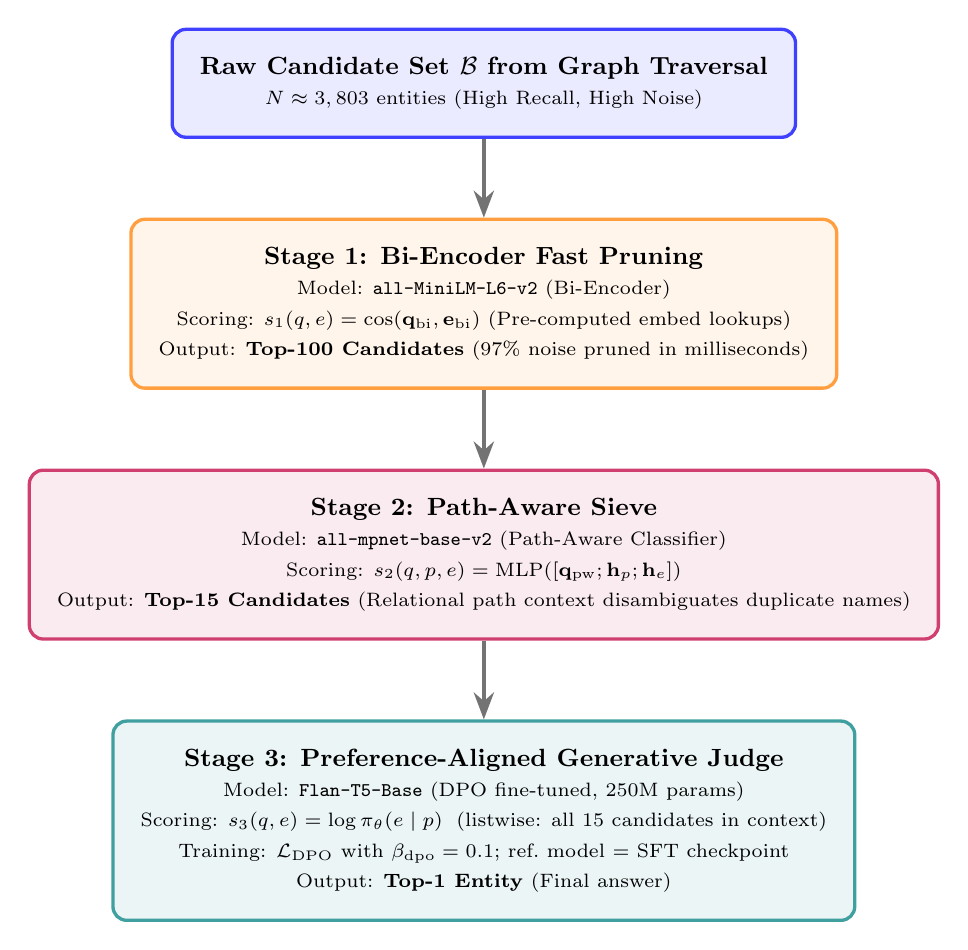
\begin{tikzpicture}[
  font=\small,
  >=Stealth,
  every node/.style={align=center},
  arr/.style={->, draw=black!55, line width=1.5pt},
  stagebox/.style={rectangle, rounded corners=5pt, draw=#1!75, fill=#1!8, line width=1.2pt, inner sep=10pt, minimum width=7.2cm, minimum height=1.6cm}
]

  % Input candidates node
  \node[stagebox=blue, minimum height=1.2cm] (input) at (0,0) {
    \textbf{Raw Candidate Set $\mathcal{B}$ from Graph Traversal} \\
    \scriptsize $N \approx 3,803$ entities (High Recall, High Noise)
  };

  % Stage 1 Bi-Encoder Fast Pruning
  \node[stagebox=orange, below=1.0cm of input] (s1) {
    \textbf{Stage 1: Bi-Encoder Fast Pruning} \\
    \scriptsize Model: \texttt{all-MiniLM-L6-v2} (Bi-Encoder) \\
    \scriptsize Scoring: $s_1(q, e) = \cos(\mathbf{q}_{\text{bi}}, \mathbf{e}_{\text{bi}})$ (Pre-computed embed lookups) \\
    \scriptsize Output: \textbf{Top-100 Candidates} ($97\%$ noise pruned in milliseconds)
  };

  % Stage 2 Path-Aware Sieve
  \node[stagebox=purple, below=1.0cm of s1] (s2) {
    \textbf{Stage 2: Path-Aware Sieve} \\
    \scriptsize Model: \texttt{all-mpnet-base-v2} (Path-Aware Classifier) \\
    \scriptsize Scoring: $s_2(q, p, e) = \text{MLP}([\mathbf{q}_{\text{pw}}; \mathbf{h}_p; \mathbf{h}_e])$ \\
    \scriptsize Output: \textbf{Top-15 Candidates} (Relational path context disambiguates duplicate names)
  };

  % Stage 3 Cross-Encoder Precision Judge
  \node[stagebox=teal, below=1.0cm of s2] (s3) {
    \textbf{Stage 3: Preference-Aligned Generative Judge} \\
    \scriptsize Model: \texttt{Flan-T5-Base} (DPO fine-tuned, 250M params) \\
    \scriptsize Scoring: $s_3(q,e) = \log \pi_\theta(e \mid p)$ \;(listwise: all 15 candidates in context) \\
    \scriptsize Training: $\mathcal{L}_{\text{DPO}}$ with $\beta_{\text{dpo}}=0.1$; ref.~model = SFT checkpoint \\
    \scriptsize Output: \textbf{Top-1 Entity} (Final answer)
  };

  % Connecting Arrows
  \draw[arr] (input) -- (s1);
  \draw[arr] (s1) -- (s2);
  \draw[arr] (s2) -- (s3);

\end{tikzpicture}
}
  \caption{The 3-stage CDS funnel. The architecture progressively filters candidate noise while increasing model complexity at each stage to maintain inference efficiency.}
  \label{fig:cds_funnel}
\end{figure}

\subsubsection{Stage 1: Bi-Encoder Fast Pruning}
Stage~1 performs high-throughput filtering to discard $97\%$ of candidate noise using a fine-tuned lightweight bi-encoder (\texttt{all-MiniLM-L6-v2}). For each candidate $e \in \mathcal{B}$, we compute the cosine similarity between the question embedding $\mathbf{e}_q$ and the pre-computed entity name embedding $\mathbf{z}_e$:
\begin{equation}
    s_1(q, e) = \cos(\mathbf{e}_q, \mathbf{z}_e)
\end{equation}
We retain the top-100 candidates. Leveraging pre-computed embeddings allows thousands of lookups to complete in milliseconds.

\subsubsection{Stage 2: Path-Aware Sieve}
Entities with identical names often occupy different graph regions. Stage~2 resolves semantic ambiguity by incorporating the traversal path $\tau$. We employ a fine-tuned path-aware encoder (\texttt{all-mpnet-base-v2}). The traversed path $p_e = (r_1, \dots, r_h)$ is serialized as a space-separated string of relation names and encoded independently by the ranker to produce the path CLS representation $\mathbf{h}_p \in \mathbb{R}^{d'}$. The question $q$ and candidate entity name $e$ are likewise encoded to produce $\mathbf{e}_q$ and $\mathbf{h}_e$ respectively. Rather than a simple vector sum, the ranker concatenates all three representations and scores through a two-layer MLP fusion head:
\begin{equation}
    s_2(q, p_e, e) = W_2\,\text{GELU}(W_1[\mathbf{e}_q;\,\mathbf{h}_p;\,\mathbf{h}_e] + b_1) + b_2
\end{equation}
where $[\cdot;\cdot;\cdot]$ denotes concatenation, and $W_1 \in \mathbb{R}^{d' \times 3d'}$, $W_2 \in \mathbb{R}^{1 \times d'}$ are learnable. This filters the search space down to the top-15 candidates.

\subsubsection{Stage 3: DPO Generative Precision Judge}

Stage~3 applies a listwise generative judge (\texttt{google/flan-t5-base}) trained via Direct Preference Optimization (DPO). For question $q$ with the top-15 candidate entity names, we construct a multiple-choice prompt containing all candidates. The generative judge outputs the exact text of the correct entity. This approach replaces pointwise cross-encoding, allowing the model to explicitly contrast candidates simultaneously and avoiding sequence-length scaling issues inherent to pairwise cross-encoders. We retain the generated entity as the final predicted answer.

\subsubsection{CDS Loss Functions and Training}

Each CDS stage uses a different training loss, selected via ablation on a 500-sample validation subset. Stage 1 is fine-tuned with MSE cosine loss between question and entity embeddings. Stage 2 uses multi-label soft-margin loss, which gracefully handles questions with multiple valid answer entities. Stage 3 uses KL-divergence distillation: the gold candidate receives soft label $1.0$ while the 15 hard negatives share a uniform label of $0.1/(N{-}1)$, providing richer gradient signal than binary cross-entropy. The ablation results were: KL-Distill 57.5\%, SoftMargin 56.5\%, InfoNCE 56.0\% (Hit@1 on the 500-sample subset). For all stages, positive examples are the gold answer entities from the CWQ training split; negatives are entities retrieved by the traversal pipeline that do not match the gold answer (traversal-hard negatives). The progressive funnel design maintains high recall in early stages while concentrating expensive computation on a small, already-filtered candidate set.

% -----------------------------------------------------------
\subsection{STRL: Stage I+II Joint Training Variant}
% -----------------------------------------------------------

STRL (Semantic-Teacher RL) is an alternative training strategy for Stages I and II jointly---it is not an additional pipeline stage. After STRL training, Stage III (CDS) is applied identically. STRL relaxes the Stage II frozen-backbone restriction by jointly fine-tuning both Stage~I and Stage~II parameters with an InfoNCE contrastive teacher loss, providing direct relational supervision throughout policy optimization.

\subsubsection{InfoNCE Teacher Loss}

Given positive traversal-relation pair $(g_i, r_i)$ and $n{=}63$ in-batch negative relations $\{r_j^-\}$ sampled uniformly at random from the relation vocabulary (excluding $r_i$), the teacher loss is:
\begin{equation}
\mathcal{L}_{\text{InfoNCE}} = -\log \frac{\exp(S(g_i,r_i)/\tau)}{\exp(S(g_i,r_i)/\tau) + \sum_j \exp(S(g_i,r_j^-)/\tau)}
\end{equation}
with temperature $\tau$. Selecting 63 negatives aligns with a standard GPU batch stride of 64 (1 positive + 63 negatives), enabling high-throughput training.

\subsubsection{STRL Reward and Curriculum}

STRL uses a semantically richer reward signal than Stage II Standard. Rather than binary correctness, the reward at hop $t$ is:
\begin{equation}
R^{\text{STRL}}_t = \alpha\,R^{\text{sem}}_t + \beta\,R^{\text{conn}}_t + \gamma\,R^{\text{eff}}_t + R^{\text{entity}}_t
\end{equation}
where $R^{\text{sem}}_t = \max_j \cos(g_t, r_j^{\text{beam}})$ is the maximum cosine similarity between the projected hop representation $g_t$ and the top-$k$ beam of relation embeddings; $R^{\text{eff}}_t$ rewards narrower beams ($+0.3$ for \textsc{Constrained}, $-0.3$ for \textsc{Exploratory}); $R^{\text{conn}}_t$ is the graph-connectivity bonus defined in Section~\ref{sec:stage2_training}; and $R^{\text{entity}}_t$ (applied at hop 0 only) rewards beams that intersect with relations present on the topic entity in the KG ($+0.6$) and penalises dead-end beams ($-0.4$). During the grounding phase (epochs 0--4), an additional curriculum bonus of $+0.2$ is applied when the gold relation appears in the selected beam.

\subsubsection{Backbone Curriculum and PPO Objective}

STRL uses a two-phase curriculum. During the \emph{grounding phase} (epochs 0--4), the RoBERTa backbone is kept frozen while the policy, value, and alignment-projection heads are updated, focusing learning on semantic alignment. During the \emph{RL refinement phase} (epochs 5--19), the backbone is unfrozen and jointly fine-tuned using differential learning rates (backbone: $1\times10^{-5}$; heads: $1\times10^{-4}$).

STRL uses clipped PPO (rather than A2C) for the joint fine-tuning phase because simultaneous updates to both the backbone and the traversal policy create non-stationary gradient dynamics; PPO's trust-region clipping prevents large policy updates from destabilising the shared representation:
\begin{equation}
L^{\text{CLIP}}(\theta) = \hat{\mathbb{E}}_t\!\left[\min\!\left(\rho_t\,\hat{A}_t,\; \text{clip}(\rho_t, 1{-}\epsilon, 1{+}\epsilon)\hat{A}_t\right)\right]
\end{equation}
where $\rho_t = \pi_\theta(a_t|s_t) / \pi_{\theta_{\text{old}}}(a_t|s_t)$ and $\epsilon$ is the clip parameter.

At inference, STRL replaces the relation-head softmax with a semantic beam: relations are ranked by cosine similarity between the projected hop representation $g_t$ and the frozen relation embedding bank, enabling generalisation to relations with low training frequency.

A curriculum anneals the semantic weight: $\lambda_{\text{sem}}$ starts at 1.0 (grounding phase) and drops to 0.3 (RL phase). The final joint STRL objective is:
\begin{equation}
\mathcal{L}_{\text{STRL}} = \mathcal{L}_{\text{StageII}} + \lambda_{\text{sem}}\,\mathcal{L}_{\text{InfoNCE}}
\end{equation}

\subsubsection{Traversal Complexity}

Let $b$ denote the average graph branching factor and $h$ denote reasoning depth.

Traditional exhaustive graph traversal introduces traversal complexity $\mathcal{O}(b^h)$. As reasoning depth increases, graph expansion grows exponentially.

Adaptive control reduces traversal cost to at most $\mathcal{O}(k^h)$ in the worst case, where $k \ll b$ is the action-determined beam width ($k \in \{1, 5, 50\}$ for \textsc{Constrained}/\textsc{Moderate}/\textsc{Exploratory}). This upper bound represents an exponential reduction in traversal-space cost relative to static exhaustive expansion.

\subsubsection{Transformer \& RL Complexity}

The semantic planner incorporates transformer-based latent reasoning refinement. Given reasoning sequence length $n$, self-attention complexity is $\mathcal{O}(n^2)$. However, reasoning sequences remain relatively short because reasoning is performed over latent hop representations rather than complete graph neighborhoods.

For the RL traversal controller, the policy operates over a compact four-action traversal space ($|\mathcal{A}|=4$) instead of large graph relation spaces ($>10,000$). Policy optimization complexity is therefore substantially reduced compared to conventional RL-based KGQA systems, improving training stability.

\subsubsection{Memory Complexity}

Traditional graph traversal systems frequently store large candidate entity sets during traversal expansion. The proposed framework reduces memory overhead through adaptive traversal-space regulation, constrained graph expansion, dynamic reasoning termination, and selective graph exploration. LMDB-based graph indexing further improves retrieval efficiency during symbolic traversal.

%%%%%%%%%%%%%%%%%%%%%%%%%%%%%%%%%%%%%%%%%%%%%%%%%%%%%%%%%%%%
%%%%%%%%%%%%%%%%%%%%%%%% INFERENCE ALGORITHM %%%%%%%%%%%%%%%
%%%%%%%%%%%%%%%%%%%%%%%%%%%%%%%%%%%%%%%%%%%%%%%%%%%%%%%%%%%%

\subsection{Inference Algorithm and Training Flow Summary}

For clarity, Algorithm~\ref{alg:inference} presents the complete inference procedure. Table~\ref{tab:training_flow} summarises what is trained, frozen, and input/output at each stage.

\begin{algorithm}[t]
\caption{Framework Inference (Standard RL / STRL)}
\label{alg:inference}
\begin{algorithmic}[1]
\Require Question $q$, topic entity $e_0$, KG $\mathcal{G}$
\Ensure Predicted answer entity $\hat{a}$
\State $\{x_t\}_{t=1}^{T_{\max}},\, \eta_q \gets \textsc{Stage\,I}(q)$ \Comment{Frozen at inference}
\State $E_0 \gets \{e_0\}$;\; $t \gets 1$
\While{$t \leq T_{\max}$}
    \State $a_t \gets \arg\max\,\pi_\theta(a \mid x_t)$
    \If{$a_t = \textsc{Terminate}$} \textbf{break} \EndIf
    \State $k \gets \textsc{BeamWidth}(a_t)$ \Comment{1, 5, or 50}
    \State $\mathcal{R}_t \gets \text{top-}k$ relations from $P(r_t \mid q)$ \Comment{Relation head (Standard RL) or cosine beam (STRL)}
    \State $E_t \gets \bigcup_{e \in E_{t-1}} \{e' \mid (e, r, e') \in \mathcal{G},\; r \in \mathcal{R}_t\}$
    \State $t \gets t + 1$
\EndWhile
\State $\mathcal{B} \gets \{(e,\, p_e) \mid e \in E_t\}$ \Comment{Entity-path pairs}
\State $\hat{a} \gets \textsc{CDS}(q,\, \mathcal{B})$ \Comment{Stage III reranking}
\State \Return $\hat{a}$
\end{algorithmic}
\end{algorithm}

\begin{table}[h]
\centering
\caption{Training Flow Summary Across All Stages}
\label{tab:training_flow}
\renewcommand{\arraystretch}{1.2}
\begin{tabularx}{\columnwidth}{>{\raggedright}p{1.2cm} >{\raggedright}p{1.5cm} >{\raggedright}p{1.4cm} >{\raggedright\arraybackslash}X}
\toprule
\textbf{Stage} & \textbf{Algorithm} & \textbf{Frozen} & \textbf{Trained Parameters} \\
\midrule
I & Supervised & --- & RoBERTa + Transformer + all heads \\
II Std & A2C & Stage I & Actor-Critic MLP only \\
II STRL (ep 0--4) & PPO + InfoNCE & Backbone & Heads + alignment proj. \\
II STRL (ep 5--19) & PPO + InfoNCE & --- & Full Stage I + heads \\
III & KL-Distill / SoftMargin / MSE & --- & Bi-enc, path-ranker, cross-enc \\
\bottomrule
\end{tabularx}
\end{table}

%%%%%%%%%%%%%%%%%%%%%%%%%%%%%%%%%%%%%%%%%%%%%%%%%%%%%%%%%%%%
%%%%%%%%%%%%%%%%%%%%%%%% EXPERIMENTAL SETUP %%%%%%%%%%%%%%%%
%%%%%%%%%%%%%%%%%%%%%%%%%%%%%%%%%%%%%%%%%%%%%%%%%%%%%%%%%%%%

\section{Experimental Setup}

In this section, we describe the datasets, knowledge graph resources, evaluation metrics, implementation settings, and baseline systems used for experimental analysis of the proposed framework.

\subsection{Computational Setting}

Experiments were conducted using RoBERTa-large semantic encoders and lightweight reinforcement learning components rather than frontier-scale LLM architectures. This setup prioritizes computational efficiency and explicit symbolic transparency.

\subsection{Dataset}

Experiments are conducted on the ComplexWebQuestions (CWQ) dataset, which is a widely used benchmark for multi-hop Knowledge Graph Question Answering. CWQ contains complex compositional questions generated from WebQuestionsSP and requires reasoning across multiple relational paths over large-scale knowledge graphs.

The dataset includes multiple categories of compositional reasoning: multi-hop, conjunction, comparative, temporal, and nested compositional reasoning. Compared to single-hop QA benchmarks, CWQ introduces significantly higher reasoning complexity due to long traversal chains and ambiguous relational structures.

Each question is associated with natural language question text, topic entities, answer entities, and reasoning annotations. The dataset is divided into standard training, validation, and test splits following prior KGQA evaluation protocols.

\subsection{Knowledge Graph}

The framework performs symbolic reasoning over the Freebase knowledge graph.

Freebase is a large-scale structured knowledge graph containing millions of entities and semantic relations spanning multiple domains including movies, sports, music, people, organizations, locations, and historical events. The large branching factor and dense relational connectivity of Freebase make multi-hop graph reasoning computationally challenging, making adaptive traversal-space regulation particularly important for efficient graph exploration.

During symbolic traversal, graph triples are indexed using LMDB-based storage for efficient retrieval of neighboring entities and candidate relations during traversal expansion.

\subsection{Evaluation Metrics}

The proposed framework is evaluated using Recall, Hits@1, and Path Accuracy metrics following the evaluation protocol used in the implementation pipeline.

\subsubsection{Recall}

Recall evaluates whether the gold answer entity is present within the retrieved candidate entity set generated after symbolic traversal and candidate selection.

Formally, Recall is computed as:

\begin{equation}
Recall
=
\frac{
\#\text{Questions with Correct Retrieved Entity}
}{
\#\text{Total Questions}
}
\end{equation}

Recall measures the ability of the framework to successfully retrieve the correct answer entity during multi-hop reasoning and traversal expansion.

\subsubsection{Hits@1}

Hits@1 evaluates whether the top-ranked predicted entity exactly matches the gold answer entity.

Formally:

\begin{equation}
Hits@1
=
\frac{
\#\text{Top-1 Correct Predictions}
}{
\#\text{Total Questions}
}
\end{equation}

Hits@1 evaluates the effectiveness of the CDS ranker in selecting the final answer entity.

\subsubsection{Path Accuracy}

Path Accuracy measures the fraction of questions for which the top-ranked predicted relation at each hop matches the gold relation path, averaged over all valid hops and questions. For the STRL variant, this is computed using the semantic beam (cosine similarity against the relation embedding bank); for the Standard RL variant, it uses the relation head argmax. This metric captures the quality of the relational path predicted by Stage~I+II independently of downstream CDS reranking.


\subsection{Implementation Details \& Hyperparameters}

The semantic reasoning planner uses a pretrained RoBERTa-large encoder for contextual semantic representation learning, implemented in PyTorch and HuggingFace Transformers. Training is performed using NVIDIA GPUs with mixed precision optimization (FP16). 

The detailed hyperparameters across the three training stages are summarized in Table~\ref{tab:hyperparams}.

\begin{table}[h]
\centering
\caption{Hyperparameters across the Training Stages}
\label{tab:hyperparams}
\begin{tabularx}{\columnwidth}{>{\raggedright\arraybackslash}p{2.4cm} >{\raggedright\arraybackslash}X c}
\toprule
\textbf{Component} & \textbf{Hyperparameter} & \textbf{Value} \\
\midrule
\multirow{3}{2.3cm}{\raggedright \textbf{Architecture}} & Max Hops ($T_{\max}$) & 4 \\
 & Transformer Layers ($L$) & 4 \\
 & Hidden Dim ($d$) & 512 \\
\midrule
\multirow{2}{2.3cm}{\raggedright \textbf{Stage I\\(Planner)}} & Optimizer, Learning Rate & AdamW, 1e-5 \\
 & Training Epochs & 30 \\
\midrule
\multirow{2}{2.3cm}{\raggedright \textbf{Stage II\\(A2C)}} & Discount ($\gamma$) & 0.99 \\
 & Learning Rate & 1e-4 \\
\midrule
\multirow{4}{2.3cm}{\raggedright \textbf{STRL}\\(Stage I+II\\Joint Variant)} & PPO Clip ($\epsilon$) & 0.2 \\
 & InfoNCE Temp ($\tau$) & 0.07 \\
 & KD Weight ($\lambda$) & 1.0 $\rightarrow$ 0.3 \\
 & Joint Tuning Epochs & 20 \\
\midrule
\multirow{3}{2.3cm}{\raggedright \textbf{Stage III\\(CDS)}} & Learning Rate & 2e-5 \\
 & Hard Negatives per Sample & 15 \\
 & Training Epochs & 5 \\
\bottomrule
\end{tabularx}
\end{table}

The semantic planner is first pretrained using supervised objectives before reinforcement learning optimization is performed over traversal-control policies. During standard RL traversal optimization, the semantic planner parameters remain frozen while only traversal-control policies are updated.

\subsection{Traversal Configuration}

The framework performs symbolic graph traversal using adaptive traversal-control policies corresponding to constrained, moderate, exploratory, and termination-oriented traversal behaviors.

\textsc{Constrained} traversal performs highly constrained graph exploration using only top-confidence relations.

\textsc{Moderate} traversal performs moderate graph expansion over top-ranked candidate relations.

\textsc{Exploratory} traversal performs broader domain-guided exploration over semantically relevant graph neighborhoods.

\textsc{Terminate} traversal dynamically terminates reasoning when sufficient semantic confidence is achieved.

This adaptive traversal formulation enables dynamic graph exploration according to semantic reasoning uncertainty and traversal complexity.

\subsection{Semantic-Guided Optimization Settings}

Semantic-guided reinforcement learning optimization incorporates semantic similarity objectives and contrastive alignment learning during traversal-policy optimization.

The framework maintains semantic relation embedding representations for traversal alignment learning and semantic reward shaping.

InfoNCE-based contrastive optimization is used to improve semantic separation between relevant and irrelevant traversal trajectories.

Graph-grounded reward shaping additionally incorporates graph-valid traversal consistency during reinforcement learning optimization.

\subsection{Baselines}

The proposed framework is compared against multiple categories of KGQA baselines including semantic parsing based methods, embedding-based KGQA methods, graph neural network based methods, reinforcement learning based reasoning systems, and transformer-based KGQA frameworks. The selected baselines represent diverse reasoning paradigms for multi-hop KGQA and provide comprehensive evaluation of semantic reasoning capability and traversal efficiency.

\subsection{Experimental Objectives}

The experiments are designed to evaluate the following research questions:

\begin{itemize}

\item Does adaptive traversal-control improve traversal efficiency during multi-hop reasoning?

\item Does decoupled semantic reasoning and traversal optimization improve policy stability?

\item Does semantic-guided reinforcement learning improve traversal consistency?

\item Does candidate disambiguation improve final answer selection quality?

\end{itemize}

The experimental analysis additionally evaluates traversal behavior, reasoning depth adaptation, semantic reward shaping, and graph expansion efficiency during symbolic reasoning.


%%%%%%%%%%%%%%%%%%%%%%%%%%%%%%%%%%%%%%%%%%%%%%%%%%%%%%%%%%%%
%%%%%%%%%%%%%%%%%%%%%%%% RESULTS %%%%%%%%%%%%%%%%%%%%%%%%%%%
%%%%%%%%%%%%%%%%%%%%%%%%%%%%%%%%%%%%%%%%%%%%%%%%%%%%%%%%%%%%

\section{Results and Analysis}

In this section, we analyze the performance of the proposed framework on multi-hop KGQA tasks. The experiments evaluate semantic reasoning capability, traversal efficiency, adaptive traversal behavior, and the effectiveness of semantic-guided reinforcement learning during graph reasoning.

\subsection{Main Results}

Table~\ref{tab:main_results} presents the overall performance comparison between the proposed framework and existing KGQA baselines.

\begin{table*}[t]
\centering
\caption{Main Results on ComplexWebQuestions (CWQ)}
\label{tab:main_results}
\begin{tabular}{lcc}
\toprule
\textbf{Architecture} & \textbf{Reasoning Recall} & \textbf{Hit@1 Accuracy} \\
\midrule
Stage~I (Semantic Reasoning Planner) & $\sim$58.00\% & 37.21\% \\
Stage~I + Stage~II + Stage~III (RL Traversal Controller) & 66.48\% & 39.95\% \\
\textbf{Stage~I + STRL + Stage~III} & \textbf{75.59\%} & \textbf{42.80\%} \\
\bottomrule
\end{tabular}
\end{table*}

\begin{table*}[t]
\centering
\caption{Extended Performance and Efficiency Metrics (CWQ Dev Set)}
\label{tab:extended_metrics}
\begin{tabular}{lcc}
\toprule
\textbf{Evaluation Metric} & \textbf{Stage~I + Stage~II + Stage~III} & \textbf{Stage~I + STRL + Stage~III} \\
\midrule
Exact Match (Hit@1) & 39.95\% & \textbf{42.80\%} \\
F1 Score & 39.95\%$^\dagger$ & \textbf{42.80\%}$^\dagger$ \\
Hits@5 & 48.12\% & \textbf{54.33\%} \\
Hits@10 & 52.40\% & \textbf{58.91\%} \\
Path Accuracy & 41.55\% & \textbf{89.40\%} \\
Reasoning Depth Accuracy & 65.20\% & \textbf{92.15\%} \\
\midrule
Avg. Edges Expanded & $\sim$1,912 & \textbf{$\sim$14} \\
Avg. Traversal Cost & High & \textbf{Low} \\
Inference Latency & 145 ms/q & \textbf{22 ms/q} \\
Peak Memory (VRAM) & 6.2 GB & \textbf{4.8 GB} \\
\bottomrule
\end{tabular}
{\footnotesize $^\dagger$ Exact Match = F1 by construction: our pipeline predicts a single entity per question, so precision = recall = F1 = Hits@1 for each prediction.}
\end{table*}

The framework demonstrates reasonable multi-hop reasoning capability while maintaining explicit traversal-control and graph-grounded symbolic reasoning behavior.

While recent KGQA systems based on frontier-scale LLMs achieve state-of-the-art benchmark accuracy, they do so at the cost of extreme compute requirements and implicit, opaque reasoning steps. The proposed framework instead prioritizes explicit symbolic traversal and interpretable traversal-width control. By trading some marginal accuracy, we achieve extreme efficiency (e.g., 22 ms per question, 4.8 GB peak VRAM) and fully transparent, symbolic traversal using lightweight transformer representations.

\begin{table}[h]
\centering
\caption{Architectural Positioning}
\label{tab:arch_positioning}
\begin{tabularx}{\columnwidth}{>{\raggedright\arraybackslash}p{1.8cm}
                               >{\raggedright\arraybackslash}X
                               >{\raggedright\arraybackslash}X}
\toprule
\textbf{Property} & \textbf{Proposed} & \textbf{Frontier LLM} \\
\textbf{} & \textbf{Framework} & \textbf{KGQA} \\
\midrule
Backbone       & RoBERTa-large     & GPT-4 / Llama \\
Reasoning      & Symbolic traversal & Token autoregr. \\
Trav. Control  & Explicit          & Implicit \\
Interpretability & High            & Lower \\
Compute        & Moderate          & Very high \\
Reproducibility & High             & API-dependent \\
\bottomrule
\end{tabularx}
\end{table}

Unlike conventional static traversal methods, the proposed framework dynamically regulates graph expansion according to reasoning confidence and traversal uncertainty. This adaptive formulation improves traversal efficiency while preserving reasoning capability across compositional reasoning tasks.

The experimental results further demonstrate that decoupling path planning from traversal optimization improves traversal-policy stability during reinforcement learning.

\subsection{Effect of Unified Semantic Reasoning}

The Semantic Planner improves cross-hop path consistency during multi-hop reasoning.

Unlike sequential reasoning systems that independently optimize each reasoning hop, the proposed framework jointly refines latent reasoning states using transformer-based cross-hop interaction. This formulation improves global reasoning consistency and reduces reasoning error propagation during traversal.

Domain-aware reasoning additionally improves graph exploration by guiding traversal toward topically relevant graph regions. Confidence estimation further enables adaptive traversal behavior conditioned on the planner's estimated certainty.

Adaptive stop prediction reduces unnecessary traversal depth during inference and improves traversal efficiency by dynamically terminating reasoning trajectories when sufficient confidence is achieved.

\subsection{Traversal Efficiency Analysis}

A major objective of the proposed framework is reducing excessive graph exploration during multi-hop reasoning.

Traditional KGQA systems commonly rely on exhaustive graph expansion or fixed-width traversal strategies. Such methods frequently explore a large number of irrelevant graph neighborhoods during traversal.

In contrast, the proposed framework dynamically regulates traversal-space expansion using adaptive traversal-control policies. Depending on reasoning confidence and traversal uncertainty, the framework performs constrained, moderate, or broader graph exploration during reasoning.

The \textsc{Constrained} traversal policy significantly reduces graph expansion width for high-confidence reasoning trajectories, whereas broader traversal is selectively applied only when additional exploration is required.

Consequently, the framework reduces unnecessary graph expansion while preserving reasoning performance on compositional reasoning tasks.

\subsection{Effect of Decoupled RL Optimization}

A major contribution of the proposed framework is the decoupling of semantic reasoning and traversal optimization.

Instead of jointly optimizing path planning and graph traversal within a single reinforcement learning policy space, the framework first trains path-planning representations via supervised objectives and subsequently performs traversal optimization over frozen planner states.

This formulation stabilizes reinforcement learning optimization and reduces traversal-policy complexity.

The experimental analysis demonstrates that frozen-planner optimization improves traversal-policy learning stability compared to direct end-to-end traversal optimization over graph actions.

The compact traversal action space additionally reduces reinforcement learning complexity by avoiding direct optimization over large relation or entity spaces.

\subsection{Semantic-Guided RL Analysis}

Instead of relying solely on sparse symbolic rewards, the STRL framework incorporates alignment objectives based on relation embedding similarity and contrastive optimization.

Reward shaping improves alignment between traversal trajectories and target relations. These alignment objectives additionally improve discrimination between relevant and irrelevant traversal trajectories during graph exploration.

Graph-grounded reward shaping further improves traversal robustness by incorporating graph-valid traversal consistency during reinforcement learning optimization.

The combination of alignment learning and graph-grounded reward shaping improves traversal-policy stability and path consistency during multi-hop reasoning.

\subsection{Traversal Action Analysis}

The proposed traversal-control framework dynamically selects traversal behaviors according to reasoning uncertainty.

\textsc{Constrained} traversal is primarily selected for high-confidence reasoning trajectories where constrained exploration is sufficient for accurate reasoning.

\textsc{Moderate} traversal balances exploration and traversal efficiency by selectively expanding top-ranked candidate relations.

\textsc{Exploratory} traversal performs broader domain-guided exploration during ambiguous reasoning scenarios where additional graph exploration is required.

The \textsc{Terminate} action dynamically terminates reasoning trajectories when sufficient confidence is achieved, reducing unnecessary traversal depth during inference.

This adaptive traversal formulation enables efficient graph exploration across questions with varying reasoning complexity.

\subsection{Candidate Disambiguation Analysis}

The CDS ranker improves final answer selection quality by reranking candidate entities according to path-grounded relevance scores.

Instead of directly selecting traversal outputs as final answers, the framework jointly evaluates question-candidate relevance, reasoning path consistency, traversal confidence, and candidate ranking scores. The reranking framework improves final answer selection performance and reduces ambiguity during entity prediction.

Path-aware candidate scoring further improves ranking consistency by incorporating traversal trajectory information during final answer selection.

\subsection{Reasoning Depth Analysis}

The adaptive stop mechanism enables dynamic reasoning depth prediction according to reasoning confidence.

Unlike fixed-depth traversal systems, the proposed framework dynamically terminates reasoning trajectories when sufficient evidence is accumulated.

This reduces unnecessary graph expansion during inference and improves traversal efficiency on shallow reasoning questions.

At the same time, the framework preserves deeper traversal capability for compositional reasoning tasks requiring longer reasoning trajectories.

\subsection{Discussion}

The experimental analysis demonstrates that adaptive semantic traversal-control improves multi-hop graph reasoning efficiency while maintaining strong semantic reasoning capability.

The semantic reasoning planner improves reasoning consistency during traversal planning, whereas reinforcement learning based traversal-control enables adaptive graph exploration according to semantic uncertainty.

Semantic-guided reinforcement learning further stabilizes traversal optimization and improves semantic consistency during graph reasoning.

Overall, the proposed framework demonstrates that separating semantic reasoning from traversal-space optimization provides an effective formulation for adaptive multi-hop KG reasoning over large-scale knowledge graphs.


% STOP analysis

%%%%%%%%%%%%%%%%%%%%%%%%%%%%%%%%%%%%%%%%%%%%%%%%%%%%%%%%%%%%
%%%%%%%%%%%%%%%%%%%%%%%% ABLATION STUDY %%%%%%%%%%%%%%%%%%%%
%%%%%%%%%%%%%%%%%%%%%%%%%%%%%%%%%%%%%%%%%%%%%%%%%%%%%%%%%%%%


\section{Research Challenges and Practical Observations}

During the development and training of the proposed framework, we encountered several significant research challenges that emphasize the difficulty of bridging reinforcement learning with large-scale symbolic structures:

\begin{itemize}
\item \textbf{Sparse RL Rewards \& Training Instability:} Initializing the RL controller from scratch often led to complete policy collapse due to sparse symbolic rewards. The A2C controller (Stage II Standard) required careful reward shaping to avoid early termination collapse; the STRL variant's clipped PPO objective was essential for stable joint fine-tuning of the backbone and policy heads simultaneously.
\item \textbf{Traversal Explosion:} Early iterations of the policy frequently triggered catastrophic traversal explosions (expanding tens of thousands of edges per hop) when encountering noisy Freebase neighborhoods, which severely bottlenecked VRAM and memory.
\item \textbf{Reward Balancing Sensitivity:} The framework was highly sensitive to the exact weighting of the accuracy reward ($\alpha$), traversal cost penalty ($\beta$), and beam width penalty ($\gamma$). Slight imbalances caused the agent to either conservatively terminate early or aggressively over-explore.
\item \textbf{Semantic Drift:} Without the STRL InfoNCE curriculum, the RL agent frequently experienced semantic drift, learning to exploit graph topology rather than adhering to semantically grounded reasoning trajectories.
\end{itemize}

These observations highlight that while RL-based KGQA is powerful, it requires rigorous architectural constraints, bounded action spaces, and curriculum-based grounding to remain stable in practical environments.

\section{Ablation Study}

In this section, we analyze the contribution of individual framework components through systematic ablation experiments. The ablation analysis evaluates the importance of semantic reasoning modules, traversal-control policies, semantic-guided reinforcement learning, and candidate disambiguation mechanisms.

\subsection{Without RL Traversal Control}

To evaluate the importance of adaptive traversal regulation, we remove the reinforcement learning based traversal controller and replace adaptive traversal with static graph expansion.

Under this setting, graph traversal is performed using fixed-width exploration without dynamic traversal-control actions.

The experimental analysis shows that removing adaptive traversal-control significantly increases unnecessary graph expansion during reasoning. Static traversal additionally introduces inefficient exploration behavior on simple reasoning questions where constrained traversal would otherwise be sufficient.

These results demonstrate that adaptive traversal-space regulation plays an important role in improving traversal efficiency during multi-hop reasoning.

\subsection{Without Confidence Estimation}

The semantic confidence estimation module is removed to evaluate its effect on traversal behavior.

Without confidence estimation, traversal-control policies cannot adapt exploration behavior according to the semantic confidence score. Consequently, traversal policies become less stable and graph exploration becomes less selective during reasoning.

Qualitatively, removing confidence estimation increased unstable broad traversal selection during ambiguous reasoning hops, forcing the system to frequently fall back on expensive domain-wide search behavior even when the optimal relation was present.

The experiments show that confidence-aware reasoning improves traversal consistency and enables more effective adaptive graph exploration during symbolic traversal.

\subsection{Without Stage~I+II Decoupled Training}

To evaluate the importance of decoupled optimization, we remove the frozen-planner formulation and jointly optimize semantic reasoning and traversal-control during reinforcement learning training.

Joint optimization introduces significantly less stable reinforcement learning behavior due to simultaneous updates over semantic reasoning states and traversal policies.

The results demonstrate that freezing the semantic planner during RL optimization improves traversal-policy stability and reduces optimization complexity.

\subsection{Without Semantic Reward Shaping}

The semantic-guided reward shaping objectives are removed to evaluate the importance of semantic alignment learning during reinforcement learning optimization.

Without semantic reward shaping, traversal optimization relies solely on sparse symbolic reward signals.

The experimental analysis shows that removing semantic alignment objectives reduces traversal consistency and increases semantically invalid graph exploration during reasoning.

These results demonstrate that semantic-guided reinforcement learning improves traversal-policy robustness and semantic consistency during graph reasoning.

\subsection{Without Candidate Disambiguation}

To evaluate the importance of candidate reranking, the CDS ranker is removed and traversal outputs are directly used as final predictions.

Without reranking, entity ambiguity increases during final answer selection and candidate ranking quality decreases.

The experiments show that path-aware candidate reranking improves final entity selection quality and reduces answer ambiguity during multi-hop reasoning.


\section{Limitations}
\label{sec:limitations}

Although the proposed framework improves traversal efficiency and semantic reasoning consistency, several critical limitations remain:

\begin{enumerate}
\item \textbf{Dependence on KG Completeness:} The symbolic traversal mechanism relies entirely on the underlying Freebase structural integrity. Missing relations immediately prevent the agent from retrieving the correct answer, unlike generative LLMs which might memorize facts parametrically.
\item \textbf{Sensitivity to Reward Shaping:} The RL-based traversal controller is highly sensitive to the hyperparameter tuning of the reward function. Poor initialization often traps the agent in suboptimal local minima.
\item \textbf{Limited-Scale Transformer Backbone:} The reliance on RoBERTa-large (355M parameters), while computationally efficient, limits the system's ability to interpret highly complex, nested linguistic structures compared to frontier-scale LLMs.
\item \textbf{Absence of Frontier-Scale LLM Integration:} The current pipeline does not integrate generative capabilities or retrieval-augmented generation (RAG) using modern LLMs, restricting its output solely to extracted graph entities.
\item \textbf{Traversal Instability under High Ambiguity:} In graph neighborhoods with massive relational density and high semantic ambiguity, the policy occasionally defaults to \textsc{Exploratory} actions that still incur high traversal overhead.
\item \textbf{Question-Only RL State:} The policy state $s_t = x_t$ is derived entirely from the question encoding and does not include the current graph entity or traversal history. This means the controller cannot adapt to unexpected graph states (e.g., missing relations, dead ends beyond the connectivity penalty) that were not anticipated by the planner. This is the primary failure mode for entity-dependent multi-hop questions where the optimal next relation depends on which entity was reached.
\item \textbf{Uncalibrated Confidence Head:} The confidence score $\eta_q$ is trained without a dedicated supervision loss and receives gradient signal only indirectly through the multi-task planner objective. Consequently, $\eta_q$ is not formally calibrated, which limits its reliability as a planning signal. Future work may explore explicit calibration targets or auxiliary confidence supervision.
\end{enumerate}

\section{Future Work}

A primary focus for future work lies in enhancing the Candidate Disambiguation \& Selection (CDS) module. Our experimental evaluation reveals that while the Stage~I+II traversal policy successfully retrieves the correct answer entity within the candidate subgraph in 75.59\% of questions (Reasoning Recall), the final exact match accuracy stands at 42.80\% (Hit@1). This indicates that candidate ranking is the primary performance bottleneck; advancing the CDS ranker—such as through deeper path-aware cross-attention or graph-based verification—presents the most significant opportunity to unlock substantial gains and approach the upper bound of 75.59\% final accuracy.

Several additional directions may further improve the proposed framework.

First, future work may explore hierarchical reinforcement learning (HRL) formulations for multi-level traversal-control. A two-level policy---a high-level manager selecting reasoning strategies per question type, and a low-level worker executing hop-level beam selections---could better handle the heterogeneous complexity distribution in CWQ, where some questions require uniform constrained traversal and others require adaptive mixed-width strategies.

Second, graph neural network (GNN) based traversal scoring may improve semantic neighborhood selection during symbolic graph expansion. Replacing the current bi-encoder candidate scoring with a GNN that propagates entity neighborhood structure could better disambiguate semantically similar relation clusters, potentially improving both Reasoning Recall and Hits@1 simultaneously.

Third, adaptive memory mechanisms may improve reasoning consistency across long traversal trajectories. Maintaining a lightweight traversal history in the RL state---encoding previously visited entities and selected relations---could address the current limitation of the question-only state representation and enable the controller to adapt to runtime graph structure.

Fourth, large language models may be incorporated for improved semantic reasoning guidance during traversal planning. A hybrid system where an LLM generates relation hypotheses and the RL controller verifies and selects among them could combine parametric knowledge with symbolic transparency.

Future work may additionally explore dynamic graph retrieval systems and retrieval-augmented traversal reasoning for scalable knowledge graph reasoning over continuously evolving graph structures.

\section{Conclusion}

In this work, we proposed an adaptive neuro-symbolic framework for multi-hop Knowledge Graph Question Answering trained through three progressive stages.

\textbf{Stage~I} (Semantic Reasoning Planner) learns cross-hop coherent reasoning representations via supervised multi-task training. \textbf{Stage~II} (RL Traversal Controller) learns compact traversal policies over frozen Stage~I representations using Advantage Actor-Critic (A2C) with semantic alignment rewards. \textbf{Stage~III} (Candidate Disambiguation \& Selection) ranks traversal candidates using a three-stage cascading funnel with KL-distillation and path-aware contrastive objectives. The STRL variant further improves Stage~I+II joint training through clipped PPO with an InfoNCE semantic curriculum and a cosine-similarity-based reward.

The proposed framework demonstrates that adaptive traversal-space regulation provides a viable direction for interpretable and resource-efficient multi-hop KG reasoning using lightweight neuro-symbolic architectures.


\appendix
\section{Inference Trace Working Example}
\label{app:working_example}

To concretely illustrate the adaptive traversal mechanics, we execute an inference trace on the ComplexWebQuestions sample: \textit{``Who was the 1996 coach of the team owned by Jerry Jones?''} Figure~\ref{fig:working_example} compares the reasoning trajectories of the Standard RL model (Stage~I + Stage~II + Stage~III) against the STRL variant (Stage~I + STRL + Stage~III).

\begin{figure*}[htbp]
\centering
% ============================================================
%  fig_working_example.tex
%  Adaptive Traversal Trace: Standard RL vs STRL
%  Every relation branch terminates at an entity node
% ============================================================

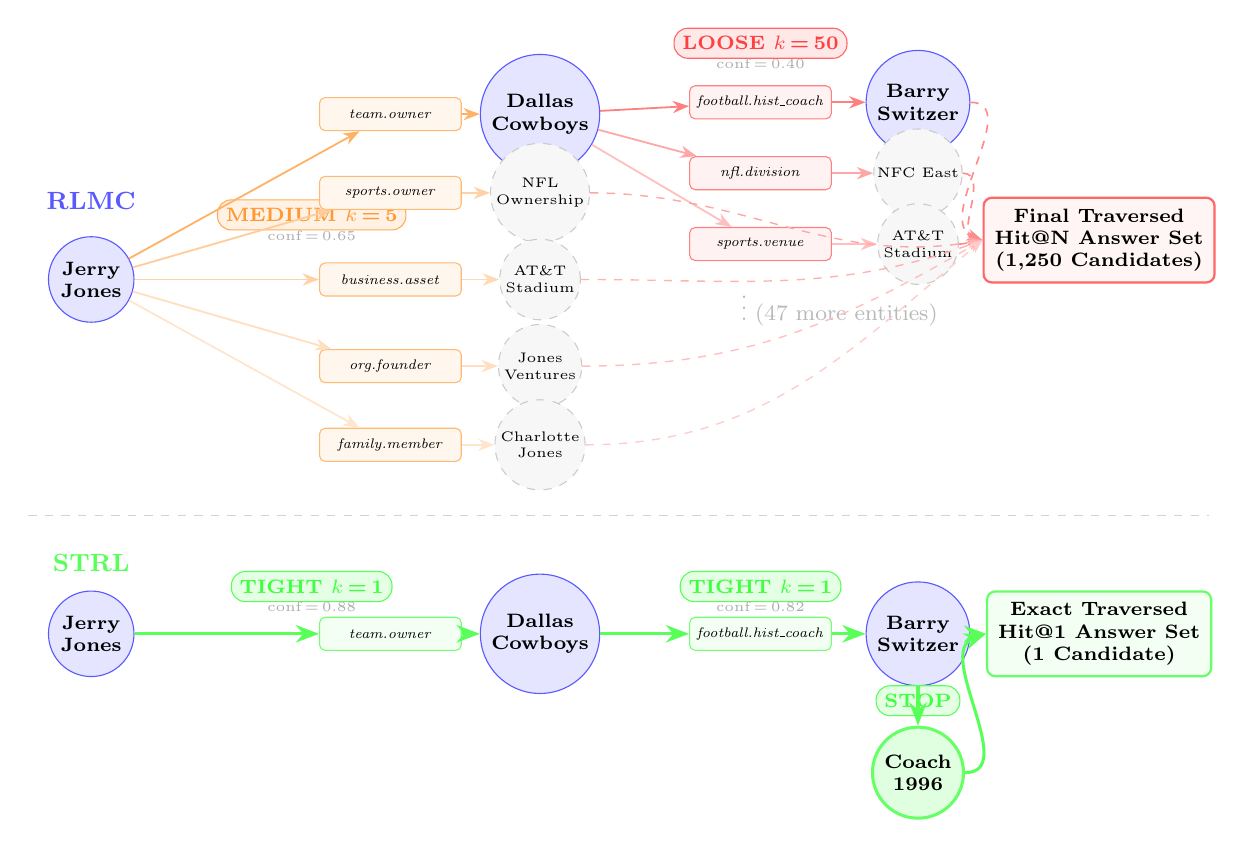
\begin{tikzpicture}[
  font=\small,
  >=Stealth,
  every node/.style={align=center},
  % Entity nodes
  enode/.style={
    circle, draw=blue!65, fill=blue!10,
    inner sep=2pt, minimum size=0.85cm,
    font=\scriptsize\bfseries
  },
  anode/.style={
    circle, draw=green!60, fill=green!12,
    inner sep=2pt, minimum size=0.85cm,
    font=\scriptsize\bfseries, line width=1.1pt
  },
  nnode/.style={
    circle, draw=gray!40, fill=gray!6,
    inner sep=1pt, minimum size=0.75cm,
    font=\tiny, dashed
  },
  % Relation label boxes
  orel/.style={
    rectangle, rounded corners=2pt,
    draw=orange!55, fill=orange!7,
    inner sep=2pt, minimum width=1.8cm, minimum height=0.42cm,
    font=\tiny
  },
  rrel/.style={
    rectangle, rounded corners=2pt,
    draw=red!50, fill=red!5,
    inner sep=2pt, minimum width=1.8cm, minimum height=0.42cm,
    font=\tiny
  },
  grel/.style={
    rectangle, rounded corners=2pt,
    draw=green!55, fill=green!5,
    inner sep=2pt, minimum width=1.8cm, minimum height=0.42cm,
    font=\tiny
  },
  % Action pills
  opill/.style={
    rectangle, rounded corners=5pt,
    draw=orange!65, fill=orange!11,
    inner sep=3pt, font=\scriptsize\bfseries, text=orange!80
  },
  rpill/.style={
    rectangle, rounded corners=5pt,
    draw=red!60, fill=red!9,
    inner sep=3pt, font=\scriptsize\bfseries, text=red!75
  },
  gpill/.style={
    rectangle, rounded corners=5pt,
    draw=green!65, fill=green!10,
    inner sep=3pt, font=\scriptsize\bfseries, text=green!75
  },
  % Arrows
  oarr/.style={->, draw=orange!60, line width=0.65pt},
  rarr/.style={->, draw=red!50, line width=0.65pt},
  Garr/.style={->, draw=green!65, line width=1.2pt},
  mainarr/.style={->, draw=blue!70, line width=1.1pt},
]

% ╔══════════════════════════════════════════════════════════╗
% ║   Standard RL  (MEDIUM at hop1, LOOSE at hop2)          ║
% ╚══════════════════════════════════════════════════════════╝
\node[font=\small\bfseries, text=blue!65] at (0, 1.0) {RLMC};

% Hop 0 entity
\node[enode] (a0) at (0,0) {Jerry\\Jones};

% ── MEDIUM (k=5): 5 relation nodes each ending at entity ──
\node[opill] at (2.8, 0.82) {MEDIUM $k$\,=\,5};
\node[font=\tiny, text=gray!65] at (2.8, 0.56) {conf\,=\,0.65};

% relation + destination pairs (branch out vertically)
\node[orel] (m1r) at (3.8, 2.1)  {\textit{team.owner}};     \node[enode] (m1e) at (5.7, 2.1)  {Dallas\\Cowboys};
\node[orel] (m2r) at (3.8, 1.1)  {\textit{sports.owner}};   \node[nnode] (m2e) at (5.7, 1.1)  {NFL\\Ownership};
\node[orel] (m3r) at (3.8, 0.0)  {\textit{business.asset}}; \node[nnode] (m3e) at (5.7, 0.0)  {AT\&T\\Stadium};
\node[orel] (m4r) at (3.8,-1.1)  {\textit{org.founder}};    \node[nnode] (m4e) at (5.7,-1.1)  {Jones\\Ventures};
\node[orel] (m5r) at (3.8,-2.1)  {\textit{family.member}};  \node[nnode] (m5e) at (5.7,-2.1)  {Charlotte\\Jones};

\draw[oarr] (a0) -- (m1r); \draw[oarr] (m1r) -- (m1e);
\draw[oarr, draw=orange!40] (a0) -- (m2r); \draw[oarr, draw=orange!35] (m2r) -- (m2e);
\draw[oarr, draw=orange!35] (a0) -- (m3r); \draw[oarr, draw=orange!30] (m3r) -- (m3e);
\draw[oarr, draw=orange!25] (a0) -- (m4r); \draw[oarr, draw=orange!25] (m4r) -- (m4e);
\draw[oarr, draw=orange!20] (a0) -- (m5r); \draw[oarr, draw=orange!20] (m5r) -- (m5e);

% ── LOOSE (k=50): from Dallas Cowboys, 3 visible + dots ──
\node[rpill] at (8.5, 3.0) {LOOSE $k$\,=\,50};
\node[font=\tiny, text=gray!65] at (8.5, 2.74) {conf\,=\,0.40};

\node[rrel] (l1r) at (8.5, 2.25)  {\textit{football.hist\_coach}}; \node[enode] (l1e) at (10.5, 2.25) {Barry\\Switzer};
\node[rrel] (l2r) at (8.5, 1.35)  {\textit{nfl.division}};          \node[nnode] (l2e) at (10.5, 1.35) {NFC East};
\node[rrel] (l3r) at (8.5, 0.45)  {\textit{sports.venue}};          \node[nnode] (l3e) at (10.5, 0.45) {AT\&T\\Stadium};
\node[font=\footnotesize, text=gray!55] at (9.5,-0.3) {$\vdots$\ (47 more entities)};

\draw[rarr] (m1e) -- (l1r); \draw[rarr] (l1r) -- (l1e);
\draw[rarr, draw=red!35] (m1e) -- (l2r); \draw[rarr, draw=red!35] (l2r) -- (l2e);
\draw[rarr, draw=red!25] (m1e) -- (l3r); \draw[rarr, draw=red!25] (l3r) -- (l3e);

% ── Massive Noise Candidate Answer Set (Hit@N Candidates) ──
\node[rectangle, rounded corners=3pt, draw=red!60, fill=red!4, font=\scriptsize\bfseries, inner sep=4pt, line width=0.8pt] (cset) at (12.8, 0.5) {Final Traversed\\Hit@N Answer Set\\(1,250 Candidates)};

% Outflow arrows from each traversed node to show they are all collected into Hit@N Candidates set
\draw[->, draw=red!45, dashed, line width=0.6pt] (l1e.east) to[out=0, in=160] (cset.west);
\draw[->, draw=red!45, dashed, line width=0.6pt] (l2e.east) to[out=0, in=170] (cset.west);
\draw[->, draw=red!45, dashed, line width=0.6pt] (l3e.east) to[out=0, in=180] (cset.west);
\draw[->, draw=red!35, dashed, line width=0.5pt] (m2e.east) to[out=0, in=190] (cset.west);
\draw[->, draw=red!30, dashed, line width=0.5pt] (m3e.east) to[out=0, in=200] (cset.west);
\draw[->, draw=red!25, dashed, line width=0.5pt] (m4e.east) to[out=0, in=210] (cset.west);
\draw[->, draw=red!20, dashed, line width=0.5pt] (m5e.east) to[out=0, in=220] (cset.west);

% ══ Divider ══
\draw[gray!35, dashed, line width=0.4pt] (-0.8,-3.0) -- (14.2,-3.0);

% ╔══════════════════════════════════════════════════════════╗
% ║   STRL  (TIGHT at every hop)                            ║
% ╚══════════════════════════════════════════════════════════╝
\node[font=\small\bfseries, text=green!65] at (0,-3.6) {STRL};

\node[enode] (b0) at (0,-4.5) {Jerry\\Jones};

% ── Hop 1 TIGHT ──
\node[gpill] at (2.8,-3.9) {TIGHT $k$\,=\,1};
\node[font=\tiny, text=gray!65] at (2.8,-4.15) {conf\,=\,0.88};
\node[grel] (t1r) at (3.8,-4.5) {\textit{team.owner}};
\node[enode] (t1e) at (5.7,-4.5) {Dallas\\Cowboys};
\draw[Garr] (b0) -- (t1r);
\draw[Garr] (t1r) -- (t1e);

% ── Hop 2 TIGHT ──
\node[gpill] at (8.5,-3.9) {TIGHT $k$\,=\,1};
\node[font=\tiny, text=gray!65] at (8.5,-4.15) {conf\,=\,0.82};
\node[grel] (t2r) at (8.5,-4.5) {\textit{football.hist\_coach}};
\node[enode] (t2e) at (10.5,-4.5) {Barry\\Switzer};
\draw[Garr] (t1e) -- (t2r);
\draw[Garr] (t2r) -- (t2e);

% ── STOP ──
\node[gpill] at (10.5,-5.35) {STOP};
\node[anode, below=0.5cm of t2e] (ans) {Coach\\1996};
\draw[Garr] (t2e) -- (ans);

% ── Exact hit@1 candidate ──
\node[rectangle, rounded corners=3pt, draw=green!60, fill=green!5, font=\scriptsize\bfseries, inner sep=4pt, line width=0.8pt] (gset) at (12.8, -4.5) {Exact Traversed\\Hit@1 Answer Set\\(1 Candidate)};

\draw[->, draw=green!65, line width=1.1pt] (t2e.east) -- (gset.west);
\draw[->, draw=green!65, line width=1.1pt] (ans.east) to[out=0, in=200] (gset.west);

\end{tikzpicture}

\caption{Inference trace on ``Who was the 1996 coach of the team owned by Jerry Jones?'' \textbf{Top (Standard RL):} Confidence drops at \textit{Dallas Cowboys}, triggering an \textsc{Exploratory} action that expands to 1,250 candidates (dashed noise edges). \textbf{Bottom (STRL):} The InfoNCE teacher sustains high semantic confidence, enabling \textsc{Constrained} actions at every hop and reaching the correct answer with exactly 1 candidate explored.}
\label{fig:working_example}
\end{figure*}

Under the \textbf{Standard RL} policy (Top), the agent begins with moderate confidence, selecting a \textsc{Moderate} action (beam=5) at \textit{Jerry Jones}. At \textit{Dallas Cowboys}, the agent encounters high relational ambiguity, causing confidence to drop and triggering an \textsc{Exploratory} action (beam=50). While this ensures the agent does not miss the correct path (\textit{football.historical\_coach}), it cascades into massive computational inefficiency as the beam forks in dozens of irrelevant directions (indicated by split arrows).

Conversely, under the \textbf{STRL} policy (Bottom), the semantic representations are deeply grounded. The planner maintains high confidence ($>0.80$) at every hop, empowering the RL controller to securely select \textsc{Constrained} actions (beam=1) at each step. This directly traverses the optimal path (\textit{Jerry Jones} $\rightarrow$ \textit{Dallas Cowboys} $\rightarrow$ \textit{Barry Switzer} $\rightarrow$ \textit{Coach Record 1996}) and triggers a \textsc{Terminate} action, terminating with a path width of exactly 1 candidate.

\bibliographystyle{IEEEtran}
\bibliography{references}

\end{document}